\chapter{Periodic Structure of Calendar Systems}
\label{chap:calendar-periodic}
\markboth{Periodic Structure of Calendar Systems}{Periodic Structure of Calendar Systems}

\begin{remark}[Periodicity decision for the target of this chapter (citation)]\label{rem:calendar_ps_hook}
When this chapter decides whether a research target is periodic, determines its period type, or seeks its minimal positive period, reference is always made to the `Periodic Systems' chapter:
for the periodicity criterion see \cref{thm:ps_periodicity_decision},
for the discrimination of period types see \cref{def:ps_period_type}, \cref{prop:ps_type_discrimination},
for the search for the minimal positive period see \cref{def:ps_minimal_period_algorithm}, \cref{thm:ps_minimal_period_correctness},
and for the construction of period series and epicycle groups from data see \cref{thm:ps_series_reconstruction}, \cref{def:ps_epicycle_group}.
\end{remark}

\begin{remark}[Positioning of this chapter: developed along the five-step interface of the `Periodic Systems' chapter]\label{rem:calendar_chapter_positioning}
The periodic structure of calendar systems studies the mathematical characterisation of the nesting and coordination of multiple periods in astronomical calendars. This chapter does not establish a separate periodicity criterion; instead it connects calendar systems to the five-step interface prescribed by the `Periodic Systems' chapter:
\begin{enumerate}[label=(\arabic*)]
    \item \textbf{Decision}: reduce the sexagenary sequence, the solar-term sequence, the synodic-month sequence and the tropical-year sequence to discrete dynamical systems, cite \cref{thm:ps_periodicity_decision} to decide whether they are periodic, and determine the period type;
    \item \textbf{Construction}: from solar-term data, synodic data and sexagenary data, construct the amplitude series, the frequency series and the phase series, and assemble them into a calendar epicycle group;
    \item \textbf{Adjustment}: dynamically adjust the calendar epicycle group by intercalation windows, best continued-fraction approximation and the decrease of the residual energy;
    \item \textbf{Convolution}: introduce amplitude convolution, phase convolution and frequency convolution on the calendar epicycle group, and connect them with the solar-term phase, the synodic phase and the sexagenary phase;
    \item \textbf{Integration}: connect to the tool chains of the three chapters `Discrete Sampling and Intercalation of Periodic Signals', `Harmonic Analysis' and `Time Series Analysis', forming a calendar periodicity diagnostic procedure.
\end{enumerate}
The calendrical and mathematical knowledge used in this chapter includes: the epoch systems of the *Huainanzi* `Tianwenxun' and of the *Huangji Jingshi*, the twenty-four solar terms and mid-qi, the synodic month, the sexagenary cycle, the yuan-hui-yun-shi cycles, continued fractions and best rational approximation, least common multiples and commensurability, the bounded intercalation error theorem, the Maya calendar, the Yi ten-month solar calendar and the ancient Indian lunisolar calendar.
\end{remark}

\begin{remark}[Guide to the seven themes of this chapter]\label{rem:calendar_seven_themes}
Translation---the ordering advance of the sexagenary sequence (the translation transformation of the absolute sequence and the relative sequence, \cref{prop:abs_rel_conversion});
Scaling---the fixed-length scaling of the tropical year and the synodic month (\(T_{\text{trop}}=365.2422\) days, \(T_{\text{syn}}=29.5306\) days, \cref{def:fixed_length});
Rotation---the rotational distribution of the solar terms on the ecliptic (the \(2\pi\) rotation of the phase angle and the solar ecliptic longitude, \cref{tab:jieqi_sequence});
Balance---the ordering and fixed-length constraints of intercalation (\cref{thm:calendar_stability});
Symmetry---the solar--lunar symmetry of the lunisolar calendar (the binary structure of the solar calendar and the lunar calendar, \cref{thm:lunisolar_grammar_unity});
Closure---the closure of the sixty-step cycle of the stems and branches (the sexagenary cycle, \cref{thm:yibu_ganzhi_shift});
Period---the tropical year (\(365.2422\) days), the synodic month (\(29.5306\) days) and the sexagenary cycle (\cref{def:fixed_length}).
\end{remark}

\section{Periodicity decision for calendar targets: the first step of the `Periodic Systems' chapter}
\label{sec:calendar_periodicity_decision}

\subsection{Calendar targets, decision input and decision map}

\begin{definition}[Calendar targets and decision input]\label{def:calendar_target}
A \textbf{calendar target} is one of the following objects:
\begin{enumerate}[label=(\roman*)]
    \item an ordering system of calendar units, whose state space is the sequence set \(\mathcal S=\mathbb Z\) and whose evolution map is the \(+1\) advance;
    \item a solar-term sequence or a synodic-month sequence, whose state space is a phase set;
    \item a sexagenary periodic system, whose state space is the cyclic group \(C_{60}\);
    \item a multi-period coupled system, whose state space is \(\mathbb Z_T\times\mathbb Z_S\times\cdots\).
\end{enumerate}
The \textbf{decision input} of a calendar target is the ordered pair
\[
\mathcal D_{\mathrm{L}}=(\mathcal S,\Phi),
\]
where \(\mathcal S\) is the set of calendar units and \(\Phi:\mathcal S\to\mathcal S\) is the evolution map induced by ordering advance, solar-term rotation or sexagenary cycling. If \(\mathcal S\) is a finite set, the target is called a \textbf{finite calendar target}; if \(\mathcal S\) is an infinite set, the target is called an \textbf{infinite calendar target}.
\end{definition}

\begin{definition}[Calendar decision map]\label{def:calendar_periodization}
Let a calendar target be given by the decision input \(\mathcal D_{\mathrm{L}}=(\mathcal S,\Phi)\). If the state or the output of the target is generated by the iteration of \(\Phi\), that is, if there exists \(x_0\in\mathcal S\) such that
\[
x_t=\Phi^t(x_0),\qquad t\in\mathbb Z,
\]
then \(\Phi\) is called the \textbf{calendar decision map} of the target. The calendar target is then reduced to a discrete dynamical system \((\mathcal S,\Phi)\), to which the criteria of the `Operations and Periodicity' chapter and of the `Periodic Systems' chapter may be applied directly.
\end{definition}

\begin{theorem}[Calendar periodicity decision theorem]\label{thm:calendar_periodicity_decision}
Let the decision map of a calendar target be \(\Phi\), and let \((\mathcal S,\Phi)\) be a discrete dynamical system. Then:
\begin{enumerate}[label=(\Alph*)]
    \item \textbf{Sufficient decision}: if there exists \(m\in\mathbb N^+\) such that \(\Phi^m=\mathrm{id}\), then the target is a uniformly periodic calendar system; every orbit is closed and the length of each orbit divides \(m\).
    \item \textbf{Equivalence of the decision}: the target is a uniformly periodic calendar system if and only if \(\operatorname{ord}(\Phi)<\infty\).
    \item \textbf{Pointwise criterion}: the orbit of the target at the state \(x_0\) is closed if and only if \(x_0\) is a periodic point; in that case the length of the orbit is the period at that point.
    \item \textbf{Non-omissibility}: the conjunction of conserved quantities and the symmetry group cannot replace \(\operatorname{ord}(\Phi)<\infty\); a quasi-periodic calendar target is not a periodic calendar system.
\end{enumerate}
\end{theorem}

\begin{proof}
The \cref{thm:calendar_periodicity_decision} of this chapter is the domain instantiation of \cref{thm:ps_periodicity_decision} in the `Periodic Systems' chapter:
it suffices to replace the decision map $f$ and the evolution group by the $\Phi$ of this chapter, and the four parts (A) sufficient decision, (B) equivalence of the decision, (C) pointwise criterion and
(D) non-omissibility then hold one by one. By the convention of \cref{rem:ps_applications_hook}, they are not expanded again here.
\end{proof}

\begin{corollary}[Calendar period types]\label{cor:calendar_period_type}
After the decision by \cref{thm:calendar_periodicity_decision}, a calendar target falls into one of the following types:
\begin{enumerate}[label=(\roman*)]
    \item \textbf{Trivially periodic type}: the least period is \(m_0=1\) and the state is a fixed point;
    \item \textbf{Strictly periodic type}: \(1<m_0<\infty\) and the state is strictly periodic (for example the sexagenary cycle with \(m_0=60\));
    \item \textbf{Uniformly periodic type}: \(\operatorname{ord}(\Phi)=m<\infty\) and all orbit lengths divide \(m\);
    \item \textbf{Quasi-periodic type}: \(\operatorname{ord}(\Phi)=\infty\); the orbit is not closed but is dense on a compact carrier structure (for example a lunisolar calendar without intercalation);
    \item \textbf{Eventually periodic type}: there exists \(N\) such that the target is periodic for \(t\ge N\);
    \item \textbf{Discretely periodic type}: the carrier structure is \(\mathbb Z\) and the normalised period ratio satisfies \(\rho=T_x/\Delta x\in\mathbb Q\).
    \item \textbf{Asymptotically periodic (damped) type}: the orbit is not closed, but tends asymptotically to a closed orbit or to a fixed point, the residual decaying as \(e^{-\kappa t}\) (see \cref{def:ps_period_type}(vii)).
\end{enumerate}
Here (i)--(iii) and (vi) are periodic calendar systems; (iv) is not a periodic calendar system, but may be handled with the bounded-approximation tools of intercalation; (v) is a periodic calendar system only in its stable stage; (vii), like (iv), is a type in the limiting sense; it is not a periodic calendar system and can be handled with bounded-approximation tools only in its stable stage.
\end{corollary}

\begin{proof}
Each item follows by substituting the calendar target into \cref{thm:calendar_periodicity_decision} and \cref{def:ps_period_type} of the `Periodic Systems' chapter.
\end{proof}

\begin{lemma}[Periodicity decision for the sexagenary sequence]\label{lem:ganzhi_period}
Let the state translation of the sexagenary sequence be \(\Phi:n\mapsto n+1\pmod{60}\). Then:
\begin{enumerate}[label=(\roman*)]
    \item \(\Phi\) is a cyclic translation on \(C_{60}\), with period \(60\);
    \item the state space \(C_{60}\) is a single orbit, and every non-trivial invariant must be constant;
    \item the sexagenary cycle constitutes a faithful action of \(C_{60}\), and \(60\) is the least positive period.
\end{enumerate}
\end{lemma}

\begin{proof}
(i) \(\Phi^{60}=\operatorname{id}\), and for every \(k<60\), \(\Phi^k\neq\operatorname{id}\), hence \(\operatorname{ord}(\Phi)=60\).
(ii) \(C_{60}\) is a single orbit under \(\Phi\); by \cref{thm:period_not_imply_conservation} of the `Operations and Periodicity' chapter, every conserved quantity must be constant.
(iii) This follows from (i) and (ii).
\end{proof}

\begin{lemma}[Periodicity decision for the solar-term sequence]\label{lem:jieqi_period}
Let the state translation of the solar-term sequence be \(\Phi:n\mapsto n+1\pmod{24}\). Then the solar-term sequence has period \(24\) (one year), and the twenty-four solar terms constitute a faithful action of \(C_{24}\).
\end{lemma}

\begin{proof}
Exactly \(24\) solar terms occur in one year (Definition \ref{def:jieqi_zhongqi}), hence \(\Phi^{24}=\operatorname{id}\). If \(k<24\) satisfies \(\Phi^k=\operatorname{id}\), then the \((k+1)\)-th solar term coincides with the first, contradicting the fact that the twenty-four solar terms in Table \ref{tab:jieqi_sequence} are pairwise distinct. Hence \(\operatorname{ord}(\Phi)=24\).
\end{proof}

\begin{lemma}[Periodicity decision for the synodic-month sequence]\label{lem:synodic_month_period}
The synodic-month sequence does not constitute a strictly periodic sequence---\(\operatorname{ord}(\Phi)=\infty\), since \(T_{\text{trop}}/T_{\text{syn}}\notin\mathbb Q\) (an \textbf{empirical observation / research programme}; see \cref{prop:length_incommensurability}). The synodic-month sequence is of quasi-periodic type and requires intercalation in order to achieve bounded approximation.
\end{lemma}

\begin{proof}
If there exist integers \(p,q\) such that \(p\,T_{\text{trop}}=q\,T_{\text{syn}}\) holds exactly, then \(T_{\text{trop}}/T_{\text{syn}}=q/p\in\mathbb Q\). But by the \textbf{empirical observation / research programme} of \cref{prop:length_incommensurability}, within the current precision of measurement \(T_{\text{trop}}/T_{\text{syn}}\approx 12.36827\) agrees with no \(p/q\) of bounded denominator, a contradiction. Hence, within measurable precision, the synodic month and the tropical year are incommensurable and the synodic-month sequence has no strict period. This must not be written as `by \cref{prop:length_incommensurability} it follows that \(T_{\text{trop}}/T_{\text{syn}}\) is irrational': the irrationality of a ratio of astronomical constants cannot be proved from measurement data.
\end{proof}

\begin{definition}[Algorithm for the least positive period of a calendar target]\label{def:calendar_minimal_period_algorithm}
\textbf{Input}: calendar target samples \(x_0,\dots,x_{N-1}\) and a tolerance \(\varepsilon\ge0\).
\textbf{Output}: the least positive period \(T_0\), or the verdict `not periodic'.
\textbf{Steps}:
\begin{enumerate}[label=(\arabic*)]
    \item take the candidate set \(\mathcal P=\{T\in\mathbb N^+:2T\le N\}\) and traverse it in increasing order of \(T\);
    \item for each \(T\) compute the maximum deviation
    \[
    E(T)=\max_{0\le n<N-T}\|x_{n+T}-x_n\|;
    \]
    \item output the first \(T\) satisfying \(E(T)\le\varepsilon\) as \(T_0\); if the traversal is exhausted with no solution, output `not periodic';
    \item commensurability check: use \(\rho=T_x/\Delta x\) (with \(T_0=p\) when \(\rho=p/q\) is in lowest terms; write \(\ell=T_0\Delta x=qT_x\) for the continuous span corresponding to \(T_0\) sampling points) together with \cref{prop:commensurability_periodicity_parallel} and \cref{cor:sampling_period_relation_parallel} of the `Discrete Sampling and Intercalation of Periodic Signals' chapter to check the conversion relation between \(T_0\) and the continuous period \(T_x\).
\end{enumerate}
\end{definition}

\begin{theorem}[Correctness of the algorithm for the least positive period of a calendar target]\label{thm:calendar_minimal_period_correctness}
\begin{enumerate}[label=(\roman*)]
    \item If the samples form a strictly periodic sequence with \(\varepsilon=0\) and \(N\ge2T_0\), then the algorithm outputs the discrete fundamental period \(T_0\).
    \item If the samples are obtained by sampling a continuous calendar target of fundamental period \(T_x\) at the sampling interval \(\Delta x\), and the normalised period ratio \(\rho=T_x/\Delta x=p/q\) is in lowest terms, then the algorithm outputs \(T_0=p\).
    \item If \(\rho\notin\mathbb Q\), then no true period exists: \(E(T)>0\) for every \(T\in\mathbb N^+\).
\end{enumerate}
\end{theorem}

\begin{proof}
The \cref{thm:calendar_minimal_period_correctness} of this chapter follows directly from the two conclusions of the `Discrete Sampling and Intercalation of Periodic Signals' chapter:
(i) by \cref{def:discrete_fundamental_period}, $T_0$ is the least positive period, hence $E(T_0)=0$, whilst for $T<T_0$ we have $E(T)>0$;
the algorithm traverses in increasing order of $T$, so the first index satisfying $E(T)=0$ is $T_0$;
(ii) and (iii) follow by substituting into \cref{prop:commensurability_periodicity_parallel}(ii)(iii). The complete argument is given in that chapter.
\end{proof}

\begin{example}[Example of a periodicity decision for the sexagenary sequence]\label{ex:calendar_ganzhi_period}
Starting from Jiazi (under the convention that Jiayin has index \(0\), Jiazi has index \(10\)), the sexagenary sequence has least period \(60\) by \cref{lem:ganzhi_period}. The state orbit has length \(60\), that is, the complete cycle `Jiazi$\to$Yichou$\to\dots\to$Guihai$\to$Jiazi'.
\end{example}

\begin{example}[Example of a periodicity decision for the solar-term sequence]\label{ex:calendar_jieqi_period}
For the solar-term sequence starting from Lichun, \cref{lem:jieqi_period} gives least period \(24\). The orbit has length \(24\), that is, the complete cycle `Lichun$\to$Yushui$\to\dots\to$Dahan$\to$Lichun'.
\end{example}

\begin{remark}[Conserved quantities do not guarantee periodicity]\label{rem:calendar_invariant_not_period}
The conserved quantities of a calendar system (such as conservation of equal intervals and conservation of fixed length) are auxiliary conditions for periodic structure, but they do not constitute sufficient conditions. For example, a lunisolar calendar without intercalation possesses conservation of the fixed length of the solar terms, yet the synodic-month sequence and the solar-term sequence are incommensurable and do not constitute a strict period. The periodic structure of a calendar must be decided by criteria such as \cref{thm:calendar_periodicity_decision} or \cref{lem:ganzhi_period}, \cref{lem:jieqi_period}.
\end{remark}

\section{Construction of the calendar period series and epicycle group: the second step of the `Periodic Systems' chapter}
\label{sec:calendar_series_construction}

\begin{definition}[Calendar amplitude series, frequency series and phase series]\label{def:calendar_series}
Let the state or output sequence of a calendar target be \(\{z_t\}\). If it can be written as
\[
z_t=\sum_k A_k e^{i(\omega_k t+\phi_k)}+\varepsilon_t,
\]
then
\[
\mathcal A_z(t)=\sum_k A_k e^{ikt},\qquad
\mathcal F_z(s)=\sum_k \omega_k s^k,\qquad
\mathcal P_z(t)=\sum_k e^{i(kt+\phi_k)}
\]
are called respectively the \textbf{amplitude series}, the \textbf{frequency series} and the \textbf{phase series} of the calendar target. The three agree with \cref{def:amplitude_series}, \cref{def:frequency_series} and \cref{def:phase_series} of the `Series and Convolution' chapter.
\end{definition}

\begin{definition}[Calendar epicycle group]\label{def:calendar_epicycle_group}
Let the period series of a calendar target be given by the amplitude series \(\{A_k\}\), the frequency series \(\{\omega_k\}\) and the phase series \(\{\phi_k\}\). For each \(k\) define the epicycle
\[
E_k:\theta\mapsto A_k e^{i(\theta+\phi_k)},\qquad \theta=\omega_k t,
\]
and call the set
\[
\mathfrak E_{\mathrm{L}}=\{(A_k,\omega_k,\phi_k)\}_{k\in\mathbb Z}
\]
the \textbf{epicycle group} of the calendar target. Its superposition is the calendar period series
\[
z_t=\sum_k E_k(\omega_k t)=\sum_k A_k e^{i(\omega_k t+\phi_k)}.
\]
\end{definition}

\begin{theorem}[Construction of the period series from calendar data]\label{thm:calendar_series_reconstruction}
Let the output of a calendar target be a finite periodic sequence of period \(N\). Then:
\begin{enumerate}[label=(\roman*)]
    \item the output can be expanded as a discrete Fourier series
    \[
    z_t=\sum_{k=0}^{N-1}c_k e^{i2\pi kt/N},\qquad
    c_k=\frac1N\sum_{t=0}^{N-1}z_t e^{-i2\pi kt/N};
    \]
    \item the amplitude series is given by \(|c_k|\), the phase series by \(\arg c_k\) and the frequency series by \(2\pi k/N\);
    \item if the output is a solar-term sequence or a sexagenary sequence, then the harmonics at the various levels correspond respectively to time scales such as the annual period, the semi-annual period, the seasonal period and the monthly period.
\end{enumerate}
\end{theorem}

\begin{proof}
(i) The discrete Fourier series of a finite periodic sequence is a standard result: the basis functions \(\{e^{i2\pi kt/N}\}_{k=0}^{N-1}\) constitute an orthogonal basis of \(\mathbb C^N\).
(ii) It is read off directly from \(c_k=A_k e^{i\phi_k}\).
(iii) For the solar-term sequence \(N=24\), the fundamental frequency corresponds to the annual period, the harmonic \(k=2\) to the semi-annual period, the harmonic \(k=4\) to the seasonal period and the harmonic \(k=12\) to the monthly period.
\end{proof}

\begin{definition}[Nominal epoch year and actual epoch year of the Xuanyuan calendar]\label{def:xuanyuan_epoch}
The Xuanyuan calendar takes the Yellow Emperor era as the origin of its year count. Let the \textbf{nominal epoch year} be the year \(2697\) BCE, which is a Jiazi year (sexagenary index \(10\)). Throughout, astronomical year numbering is used:
\[
Y_0=-2696.
\]
The sexagenary index of Jiayin is \(0\), so the \textbf{actual epoch year} is
\[
-2696+50=-2646\quad(\text{astronomical year numbering}),
\]
corresponding to the year \(2647\) BCE (a Jiayin year).
\end{definition}

\begin{definition}[Fixed length: the intrinsic period of a calendar unit]\label{def:fixed_length}
A \textbf{fixed length} is the intrinsic period length of a calendar unit:
\begin{center}
\begin{tabular}{>{\centering\arraybackslash}p{2.5cm}>{\centering\arraybackslash}p{2.5cm}>{\centering\arraybackslash}p{2.5cm}>{\centering\arraybackslash}p{3cm}}
\toprule
Calendar unit & Symbol & Fixed length & Type \\
\midrule
Tropical year & \(T_{\text{trop}}\) & \(365.2421897\) mean solar days & Solar period \\
Synodic month & \(T_{\text{syn}}\) & \(29.5305889\) mean solar days & Lunar period \\
Solar-term interval & \(\Delta T_{\text{jieqi}}\) & \(T_{\text{trop}}/24\approx 15.2184\) days & Solar period (mean solar-term method) \\
Mid-qi interval & \(\Delta T_{\text{zhongqi}}\) & \(T_{\text{trop}}/12\approx 30.4368\) days & Solar period (mean solar-term method) \\
Climate month & \(T_{\text{climate}}\) & \(14\)--\(18\) days & Solar period (true solar-term method, variable) \\
Sidereal year & \(T_{\text{sid}}\) & \(365.2563630\) mean solar days & Sidereal reference frame \\
\bottomrule
\end{tabular}
\end{center}
\end{definition}

\begin{definition}[Absolute sequence and relative sequence]\label{def:absolute_relative_sequence}
An \textbf{absolute sequence} is the continuous index of a calendar unit counted from the epoch year of the Xuanyuan calendar:
\[
S_{\text{abs}}(U)\in\mathbb Z.
\]
A \textbf{relative sequence} is the number of a calendar unit within the current period:
\[
S_{\text{rel}}(U)\in\{1,2,\dots,T\}.
\]
\end{definition}

\begin{proposition}[Conversion between the absolute sequence and the relative sequence]\label{prop:abs_rel_conversion}
Let the absolute sequence of a calendar unit \(U\) be \(S_{\text{abs}}(U)\), its relative sequence be \(S_{\text{rel}}(U)\), and the absolute sequence of the starting point of the current period be \(S_{\text{abs}}(P)\). Then
\[
S_{\text{rel}}(U)=S_{\text{abs}}(U)-S_{\text{abs}}(P)+1.
\]
\end{proposition}

\begin{proof}
The relative sequence is counted from \(1\) and the absolute sequence from \(S_{\text{abs}}(P)\), and the translation \(S_{\text{abs}}(P)-1\) depends only on the choice of the starting point of the period. Hence \(S_{\text{rel}}(U)=S_{\text{abs}}(U)-S_{\text{abs}}(P)+1\).
\end{proof}

\begin{proposition}[Calculation of the absolute sequence of a solar term]\label{prop:jieqi_absolute_sequence}
The absolute sequence of the \(n\)-th solar term (counted from Lichun of the epoch year) is \(S_{\text{abs}}(J_n)=n\). The corresponding year is \(Y(J_n)=Y_0+\lfloor (n-1)/24\rfloor\). The relative sequence is
\[
S_{\text{rel}}(J_n)=\bigl((n-1)\bmod 24\bigr)+1.
\]
\end{proposition}

\begin{proof}
By Definition \ref{def:absolute_relative_sequence}, the absolute sequence is the continuous numbering counted from the epoch year; Lichun of the epoch year is the first solar term, so the absolute sequence of the \(n\)-th solar term is exactly \(S_{\text{abs}}(J_n)=n\). Since one tropical year contains exactly \(24\) solar terms (Definition \ref{def:jieqi_zhongqi}), the \(n\)-th solar term falls in the \(\lfloor (n-1)/24\rfloor+1\)-th tropical year counted from the epoch year, hence \(Y(J_n)=Y_0+\lfloor (n-1)/24\rfloor\). The relative sequence is computed from \cref{prop:abs_rel_conversion}: taking the starting point \(P\) of the current period to be Lichun of that year, whose absolute sequence is \(S_{\text{abs}}(P)=24\lfloor (n-1)/24\rfloor+1\), we obtain \(S_{\text{rel}}(J_n)=((n-1)\bmod 24)+1\).
\end{proof}

\section{Dynamic adjustment of the calendar epicycle group: the third step of the `Periodic Systems' chapter}
\label{sec:calendar_adaptive}

\begin{definition}[Dynamic adjustment of the calendar epicycle group]\label{def:calendar_adaptive_adjustment}
Let the current calendar epicycle group be \(\mathfrak E^{(j)}\), with partial sum
\[
z^{(j)}(t)=\sum_{k\in\mathfrak E^{(j)}}A_k e^{i(\omega_k t+\phi_k)},
\]
and residual \(r^{(j)}=z-z^{(j)}\). \textbf{Dynamic adjustment} consists of two rules:
\begin{enumerate}[label=(\roman*)]
    \item \textbf{Quantity adjustment}: if the residual energy satisfies \(\|r^{(j)}\|^2>\delta\), then add one epicycle according to the peak of the residual periodogram;
    \item \textbf{Parameter adjustment}: update the parameters of the existing epicycles by regularised least squares or by the intercalation window.
\end{enumerate}
In calendar systems, quantity adjustment corresponds to adding a solar-term term, a synodic term or an intercalation term; parameter adjustment corresponds to tuning the length of the intercalation window, the pairing of solar terms with mid-qi, or the initial phase of the sexagenary cycle.
\end{definition}

\begin{proposition}[Monotonicity of quantity adjustment]\label{prop:calendar_adaptive_growth}
After the dominant-frequency component of the residual has been added as in \cref{def:calendar_adaptive_adjustment}(i), the residual energy is monotonically non-increasing:
\[
\|r^{(j+1)}\|^2\le\|r^{(j)}\|^2.
\]
\end{proposition}

\begin{proof}
By the orthogonal decomposition \(\|r^{(j)}\|^2=\|r^{(j+1)}\|^2+\|\text{the removed component}\|^2\), the inequality holds.
\end{proof}

\begin{theorem}[Convergence of dynamic adjustment]\label{thm:calendar_adaptive_convergence}
Let the calendar target be a \textbf{real-valued finite periodic sequence} of length $T_0$ ($T_0\in\mathbb N$) and let $\delta=0$. Then after at most $\lfloor T_0/2\rfloor+1$ steps of dynamic adjustment the residual is zero, and the resulting calendar epicycle group is the exact Fourier data of the target; for a \textbf{complex-valued} sequence the corresponding number of steps is at most $T_0$.
\end{theorem}

\begin{proof}
The discrete Fourier series of a \textbf{real-valued} finite periodic sequence of length $T_0$ ($T_0\in\mathbb N$) is complete on $\lfloor T_0/2\rfloor+1$ harmonics (including the constant term); a \textbf{complex-valued} sequence requires $T_0$ components. At each step one dominant frequency component of the residual is extracted as in \cref{prop:calendar_adaptive_growth} and the residual energy decreases strictly, so the residual vanishes after finitely many steps.
\end{proof}

\begin{remark}[Incommensurability of the fixed lengths (empirical observation / research programme)]\label{prop:length_incommensurability}
Whether the tropical year \(T_{\text{trop}}\) and the synodic month \(T_{\text{syn}}\) are commensurable depends on whether the ratio of two astronomical constants, \(r=T_{\text{trop}}/T_{\text{syn}}\), is rational. It must be stated here that `\(r\) is irrational' is an \textbf{empirical observation / research programme}, not a provable proposition: any measurement of finite precision yields a rational \(r\), whose continued-fraction expansion must terminate, and improved precision merely lengthens that expansion without ever proving that it fails to terminate. The inference from `the continued fraction keeps extending' to irrationality is therefore \textbf{invalid}, and the irrationality of a ratio of astronomical constants cannot be proved mathematically.
\textbf{Empirical hypothesis}: within the current precision of measurement, \(r\) agrees with no \(p/q\) of bounded denominator, and its sequence of continued-fraction convergents is stable within measurable precision:
\[
r=[12;\,2,\,1,\,2,\,1,\,1,\,17,\ldots].
\]
Under this hypothesis it may be asserted that there exist no integers \(p,q\) with \(p\,T_{\text{trop}}=q\,T_{\text{syn}}\) exactly---this is the fundamental reason why the lunisolar calendar requires intercalation. The best rational approximation to \(r\) is the continued-fraction convergent \(235/19=12.36842\ldots\), with an error of about \(0.00015\), which is precisely the approximate mechanism of `seven intercalary months in nineteen years'.
\cref{lem:synodic_month_period} (the synodic-month sequence is not strictly periodic) and \cref{thm:calendar_continued_fraction_best} (best intercalation by continued fractions) both take this empirical hypothesis as their premise; they are conditional, not unconditional, conclusions.
\end{remark}

\begin{definition}[Intercalation window and intercalation sequence]\label{def:calendar_intercalation}
Let the period ratio be \(\rho=T_{\text{trop}}/T_{\text{syn}}>0\). A sequence of integers \(\{N_m\}_{m\in\mathbb N}\) is called an \textbf{intercalation sequence} for \(\rho\) if
\[
N_m\in\{\lfloor\rho\rfloor,\lceil\rho\rceil\},\qquad
\lim_{M\to\infty}\frac1M\sum_{m=0}^{M-1}N_m=\rho.
\]
Define the \textbf{cumulative sample count}
\[
S_M=\sum_{m=0}^{M-1}N_m,
\]
and the \textbf{intercalation error}
\[
E_M=S_M-M\rho.
\]
\end{definition}

\begin{theorem}[Bounded intercalation error theorem]\label{thm:calendar_intercalation_error_bound}
Let \(\rho>0\). Then the three basic intercalation sequences satisfy:
\begin{enumerate}[label=(\roman*)]
    \item \textbf{Lower intercalation}: \(N_m^{\mathrm{floor}}=\lfloor (m+1)\rho\rfloor-\lfloor m\rho\rfloor\), \(E_M^{\mathrm{floor}}\in(-1,0]\);
    \item \textbf{Upper intercalation}: \(N_m^{\mathrm{ceil}}=\lceil (m+1)\rho\rceil-\lceil m\rho\rceil\), \(E_M^{\mathrm{ceil}}=\lceil M\rho\rceil-M\rho\in[0,1)\), and \(E_M^{\mathrm{ceil}}=0\) when \(M\rho\in\mathbb Z\);
    \item \textbf{Balanced intercalation}: \(N_m^{\mathrm{round}}=\operatorname{round}((m+1)\rho)-\operatorname{round}(m\rho)\), \(|E_M^{\mathrm{round}}|\le 1/2\).
\end{enumerate}
\end{theorem}

\begin{proof}
By the definition of lower intercalation,
\[
S_M^{\mathrm{floor}}=\sum_{m=0}^{M-1}(\lfloor (m+1)\rho\rfloor-\lfloor m\rho\rfloor)=\lfloor M\rho\rfloor,
\]
hence \(E_M^{\mathrm{floor}}=\lfloor M\rho\rfloor-M\rho=-\{M\rho\}\in(-1,0]\). The same argument gives \(E_M^{\mathrm{ceil}}=\lceil M\rho\rceil-M\rho\in[0,1)\) for upper intercalation, and \(E_M^{\mathrm{ceil}}=0\) when \(M\rho\in\mathbb Z\) (the ideal, leakage-free case). For balanced intercalation \(S_M^{\mathrm{round}}=\operatorname{round}(M\rho)\), and by the definition of \(\operatorname{round}\), \(|E_M^{\mathrm{round}}|\le 1/2\).
\end{proof}

\begin{theorem}[Best continued-fraction intercalation]\label{thm:calendar_continued_fraction_best}
Let \(\rho>0\) be irrational and let \(\{p_j/q_j\}\) be its continued-fraction convergents. Then:
\begin{enumerate}[label=(\roman*)]
    \item \textbf{Error bound}: \(|\rho-p_j/q_j|<1/(q_jq_{j+1})<1/q_j^2\);
    \item \textbf{Best-approximation property}: if \(q<q_{j+1}\), then \(|q\rho-p|\ge|q_j\rho-p_j|\);
    \item \textbf{Optimal window}: the optimal sequence of intercalation-window lengths is \(\{q_j\}\), with cumulative error \(|E_{q_j}|<1/q_{j+1}\).
\end{enumerate}
\end{theorem}

\begin{proof}
(i) and (ii) are standard results of continued-fraction theory (see \cref{thm:continued_fraction_best_approx_parallel} of the `Discrete Sampling and Intercalation of Periodic Signals' chapter).
(iii) From (i) we obtain directly \(|E_{q_j}|=|q_j\rho-p_j|<1/q_{j+1}\). By the optimality in (ii), this upper bound is the smallest among window lengths \(<q_{j+1}\).
\end{proof}

\begin{theorem}[Convergence of calendar intercalation]\label{thm:calendar_intercalation_convergence}
Let \(\rho=T_{\text{trop}}/T_{\text{syn}}\). Take the intercalation window to be the sequence of continued-fraction denominators \(\{q_j\}\). Then:
\begin{enumerate}[label=(\roman*)]
    \item the cumulative error satisfies \(|E_{q_j}|<1/q_{j+1}\to 0\);
    \item the relative error satisfies \(|E_{q_j}|/q_j<1/(q_jq_{j+1})\to 0\);
    \item the phases of the solar calendar and the lunar calendar close approximately on the scale of \(q_j\) years.
\end{enumerate}
\end{theorem}

\begin{proof}
By \cref{thm:calendar_continued_fraction_best}, \(|E_{q_j}|<1/q_{j+1}\). Since \(q_j\to\infty\), we have \(1/q_{j+1}\to 0\), so (i) holds. Part (ii) follows from \(q_j\to\infty\) and (i). Phase closure is equivalent to \(|E_{q_j}|\to 0\), which holds by (i).
\end{proof}

\begin{remark}[Boundary of dynamic adjustment]\label{rem:calendar_adaptive_boundary}
\cref{thm:calendar_adaptive_convergence} relies on a finite periodic sequence. For an incommensurable lunisolar calendar no finite epicycle group represents it exactly, and only a bounded approximation is possible. The choice of intercalation window is restricted by the continued-fraction convergents; intercalation does not eliminate the cost of incommensurability, but only reduces the error to a bounded one.
\end{remark}

\section{Calendar convolution: the fourth step of the `Periodic Systems' chapter}
\label{sec:calendar_convolution}

\begin{definition}[Calendar amplitude convolution, phase convolution and frequency convolution]\label{def:calendar_convolution_types}
Let two calendar epicycle groups be
\[
\mathfrak E=\{(A_n,\omega_n,\phi_n)\},\qquad
\mathfrak E'=\{(B_m,\nu_m,\psi_m)\}.
\]
Define:
\begin{enumerate}[label=(\roman*)]
    \item \textbf{Amplitude convolution}: \(\mathbb A_{mn}=A_nB_m\);
    \item \textbf{Phase convolution}: \(\mathbb P_{mn}=e^{i(\phi_n-\psi_m)}\);
    \item \textbf{Frequency convolution}: \(\mathbb F_{mn}=\omega_n\nu_m\);
    \item \textbf{Trend convolution}: \(\mathbb T_{mn}=A_nB_m e^{i(\phi_n-\psi_m)}=A_nB_m\mathbb P_{mn}\).
\end{enumerate}
This agrees with \cref{def:amplitude_convolution}, \cref{def:phase_convolution}, \cref{def:frequency_convolution} and \cref{def:tendency_convolution} of the `Series and Convolution' chapter.
\end{definition}

\begin{theorem}[Action of the three kinds of convolution on calendar epicycle groups]\label{thm:calendar_convolution_action}
Let the epicycle groups of two calendar targets be \(\mathfrak E\) and \(\mathfrak E'\). Then:
\begin{enumerate}[label=(\roman*)]
    \item amplitude convolution acts only on the radius;
    \item phase convolution acts only on the phase;
    \item frequency convolution acts only on the rate of rotation;
    \item trend convolution preserves both amplitude and phase.
\end{enumerate}
\end{theorem}

\begin{proof}
This is read off directly from \cref{def:calendar_convolution_types}.
\end{proof}

\begin{proposition}[Periodic-convolution generation of the sexagenary cycle]\label{prop:ganzhi_periodic_convolution}
The periodic convolution of the Heavenly-Stem period \(T_{\text{stem}}=10\) and the Earthly-Branch period \(T_{\text{branch}}=12\), after filtering by the parity-synchronisation condition \(n\equiv m\pmod 2\), yields exactly \(60\) effective phases, which constitute the sexagenary cycle.
\end{proposition}

\begin{proof}
The periodic convolution traverses \(10\times 12=120\) pairs \((n,m)\). The Yin-Yang synchronisation condition \(n\equiv m\pmod 2\) selects \(5\times 6+5\times 6=60\) pairs from the \(120\), which correspond exactly to the sexagenary cycle. By \cref{thm:epicycle_nesting_generation} of the `Periodic Systems' chapter, these \(60\) phases constitute the cyclic group \(C_{60}\).
\end{proof}

\begin{proposition}[Phase convolution of the solar terms and the synodic month]\label{prop:jieqi_synodic_phase_convolution}
The phase convolution of the solar-term sequence (period \(24\)) and the synodic-month sequence (period \(12\) or \(13\)) gives the relative relation between the solar-term phase and the synodic phase. Intercalation by absence of a mid-term corresponds to a particular zero of the phase convolution: when the relative difference between the solar-term phase and the mid-qi phase within a synodic month exceeds the window, that month is an intercalary month.
\end{proposition}

\begin{proof}
By \cref{def:jieqi_zhongqi_dingyue}, a normal month contains exactly one solar term and one mid-qi, and the phase difference lies within the window. When a month contains only a solar term and no mid-qi, the difference between the solar-term phase and the phase of the nearest mid-qi exceeds the window, and that month is an intercalary month. The phase convolution records the relative relations of all solar-term--synodic phase pairs.
\end{proof}

\begin{remark}[Relation between calendar convolution and periodic convolution]\label{rem:calendar_convolution_relation}
Calendar convolution is not a new convolution operation, but an instance, on the calendar epicycle group, of the periodic convolution of the `Series and Convolution' chapter. Solar-term--synodic phase convolution, sexagenary periodic convolution and month--year periodic convolution are respectively the concrete manifestations in calendars of phase convolution, frequency convolution and amplitude convolution.
\end{remark}

\section{Integration with discrete sampling, harmonic analysis and time series analysis: the fifth step of the `Periodic Systems' chapter}
\label{sec:calendar_integration}

\begin{definition}[Calendar periodicity diagnostic procedure]\label{def:calendar_periodic_diagnosis}
For a given calendar system, diagnosis is carried out within the periodic-mathematics framework:
\begin{enumerate}[label=(\roman*)]
    \item \textbf{Ordering diagnosis}: compute the absolute sequence and the relative sequence and verify the translation transformation;
    \item \textbf{Fixed-length diagnosis}: compute the fixed lengths of the tropical year, the synodic month and so on, and verify incommensurability;
    \item \textbf{Intercalation diagnosis}: compute the cumulative error of the intercalation window and verify the bounded intercalation error theorem;
    \item \textbf{Phase diagnosis}: compute the relative relations among the solar-term phase, the synodic phase and the sexagenary phase.
\end{enumerate}
\end{definition}

\begin{theorem}[The calendar periodicity diagnostic procedure and its interfaces with three chapters]\label{thm:calendar_diagnosis_integration}
The four steps of \cref{def:calendar_periodic_diagnosis} connect respectively to:
\begin{enumerate}[label=(\roman*)]
    \item the `Discrete Sampling and Intercalation of Periodic Signals' chapter: \cref{def:uniform_sampling_parallel}, \cref{thm:nyquist_shannon_parallel}, \cref{thm:intercalation_leakage_suppression};
    \item the `Harmonic Analysis' chapter: \cref{def:fourier_series}, \cref{thm:parseval_fourier}, \cref{prop:twelve_to_six};
    \item the `Time Series Analysis' chapter: \cref{def:ts_period_detection}, \cref{prop:ts_period_significance}, \cref{def:ts_window_validation}.
\end{enumerate}
Hence calendar periodicity diagnosis is not an independent method, but an application of the unified tool chain of periodic mathematics to calendar systems.
\end{theorem}

\begin{proof}
The correspondence is item by item:
(i) ordering diagnosis requires sampling and spectral estimation;
(ii) the frequency decomposition and the phase kernels are found in the `Harmonic Analysis' chapter;
(iii) the periodogram peaks, the Fisher test and window-function validation are found in the `Time Series Analysis' chapter.
Hence the diagnostic procedure is a synthesis of the tool chains of the three chapters.
\end{proof}

\begin{remark}[Operational order after integration]\label{rem:calendar_integration_order}
The recommended order for an actual diagnosis is: first decide whether the calendar target is periodic (\cref{thm:calendar_periodicity_decision}); then construct the Fourier data and the epicycle group of the solar-term, synodic and sexagenary data (\cref{thm:calendar_series_reconstruction}); then optimise the parameters by the intercalation window and dynamic adjustment (\cref{thm:calendar_adaptive_convergence}, \cref{thm:calendar_continued_fraction_best}); then perform calendar convolution and analyse the phase relations (\cref{prop:ganzhi_periodic_convolution}, \cref{prop:jieqi_synodic_phase_convolution}); finally output the diagnosis as in \cref{def:calendar_periodic_diagnosis}.
\end{remark}

\section{Ordering and fixed length: basic attributes of calendar units}
\label{sec:calendar_sequence_length}

\subsection{Absolute sequence and relative sequence}

\begin{definition}[Absolute sequence]\label{def:absolute_sequence}
An \textbf{absolute sequence} is the continuous index of a calendar unit counted from the epoch year of the Xuanyuan calendar. Let the astronomical year number of the nominal epoch year be \(Y_0=-2696\) (the historical year \(2697\) BCE, a Jiazi year). For any calendar unit \(U\), its \textbf{absolute sequence} \(S_{\text{abs}}(U)\) is defined as the continuous numbering of that unit counted from the epoch year.

The absolute sequence has the following properties:
\begin{enumerate}[label=(\roman*)]
    \item \textbf{Continuous and unbroken}: it is not interrupted by changes of dynasty, changes of reign title or calendar reform.
    \item \textbf{Uniqueness}: every calendar unit has one and only one absolute sequence number.
    \item \textbf{Monotonically increasing}: it increases strictly monotonically with time.
    \item \textbf{Computable across periods}: the time interval between any two calendar units can be computed directly from the difference of their sequences.
\end{enumerate}
\end{definition}

\begin{definition}[Relative sequence]\label{def:relative_sequence}
A \textbf{relative sequence} is the number of a calendar unit within the current period:
\begin{enumerate}[label=(\roman*)]
    \item \textbf{Relative sequence of years}: counted from the first year of the current reign title.
    \item \textbf{Relative sequence of months}: counted from the first month (the Tiger month) of the current year; an intercalary month retains the number of the preceding month.
    \item \textbf{Relative sequence of solar terms}: counted from Lichun of the current year, with Lichun as \(1\) and Dahan as \(24\).
    \item \textbf{Relative sequence of days}: counted from the day of new moon (the first day) of the current month.
\end{enumerate}
The relative sequence measures the position of a calendar unit within the current period---its value depends on the choice of the starting point of the current period.
\end{definition}

\subsection{Fixed length: the intrinsic period of a calendar unit}

\begin{remark}[The fixed-length range of the climate month]\label{rem:climate_fixed_length}
The fixed length of the climate month (Climate) is not fixed, but varies within the range \(14\)--\(18\) days. This is because, under the true solar-term method, the length of each climate month depends on the actual speed of the Sun's motion along the ecliptic---climate months near the winter solstice are shorter (about \(14\) days) and climate months near the summer solstice are longer (about \(16\)--\(18\) days). The variable fixed length of the climate month is the manifestation in the true solar-term method of the non-uniformity of the Sun's apparent motion.
\end{remark}

\begin{remark}[The mathematical significance of incommensurability]\label{rem:incommensurability_meaning}
The \textbf{empirical observation / research programme} of \cref{prop:length_incommensurability} shows that, within the current precision of measurement, the periods of the solar calendar and the lunar calendar cannot be unified exactly by any integer ratio. Any lunisolar scheme can achieve approximate coordination of these two sets of periods only in the sense of best rational approximation. The accuracy of the approximation is given by the error of the continued-fraction convergents. The ratio \(235/19\) is a high-accuracy approximation to \(T_{\text{trop}}/T_{\text{syn}}\), with relative error about \(1.2\times 10^{-5}\), corresponding to a cumulative error of about \(0.09\) days within \(19\) years---this provides a basis of error control for the intercalation scheme of the Xuanyuan calendar.
\end{remark}

\section{The ordering and fixed length of solar terms and mid-qi}
\label{sec:jieqi_zhongqi}

\begin{definition}[Distinction between solar terms and mid-qi]\label{def:jieqi_zhongqi}
The twenty-four solar terms fall into two groups: the \(12\) \textbf{solar terms} (jie) mark the beginning of each month, and the \(12\) \textbf{mid-qi} (mid-terms) mark the midpoint of each month. Solar terms and mid-qi alternate: Lichun$\to$Yushui$\to$Jingzhe$\to$Chunfen$\to\dots\to$Xiaohan$\to$Dahan.
\end{definition}

\begin{table}[htbp]
    \centering
    \caption{The ordering and fixed length of the twenty-four solar terms}
    \label{tab:jieqi_sequence}
    \begin{tabular}{>{\centering\arraybackslash}p{1.2cm}>{\centering\arraybackslash}p{1.5cm}>{\centering\arraybackslash}p{1.5cm}>{\centering\arraybackslash}p{1.8cm}>{\centering\arraybackslash}p{2cm}>{\centering\arraybackslash}p{2.5cm}}
        \toprule
        Relative index & Name & Type & Phase angle & Solar ecliptic longitude & Month order \\
        \midrule
        \(1\) & Lichun & Solar term & \(0\) & \(315^\circ\) & Beginning of the Tiger month \\
        \(2\) & Yushui & Mid-qi & \(\pi/12\) & \(330^\circ\) & Middle of the Tiger month \\
        \(3\) & Jingzhe & Solar term & \(\pi/6\) & \(345^\circ\) & Beginning of the Rabbit month \\
        \(4\) & Chunfen & Mid-qi & \(\pi/4\) & \(0^\circ\) & Middle of the Rabbit month \\
        \(5\) & Qingming & Solar term & \(\pi/3\) & \(15^\circ\) & Beginning of the Dragon month \\
        \(6\) & Guyu & Mid-qi & \(5\pi/12\) & \(30^\circ\) & Middle of the Dragon month \\
        \(7\) & Lixia & Solar term & \(\pi/2\) & \(45^\circ\) & Beginning of the Snake month \\
        \(8\) & Xiaoman & Mid-qi & \(7\pi/12\) & \(60^\circ\) & Middle of the Snake month \\
        \(9\) & Mangzhong & Solar term & \(2\pi/3\) & \(75^\circ\) & Beginning of the Horse month \\
        \(10\) & Xiazhi & Mid-qi & \(3\pi/4\) & \(90^\circ\) & Middle of the Horse month \\
        \(11\) & Xiaoshu & Solar term & \(5\pi/6\) & \(105^\circ\) & Beginning of the Goat month \\
        \(12\) & Dashu & Mid-qi & \(11\pi/12\) & \(120^\circ\) & Middle of the Goat month \\
        \(13\) & Liqiu & Solar term & \(\pi\) & \(135^\circ\) & Beginning of the Monkey month \\
        \(14\) & Chushu & Mid-qi & \(13\pi/12\) & \(150^\circ\) & Middle of the Monkey month \\
        \(15\) & Bailu & Solar term & \(7\pi/6\) & \(165^\circ\) & Beginning of the Rooster month \\
        \(16\) & Qiufen & Mid-qi & \(5\pi/4\) & \(180^\circ\) & Middle of the Rooster month \\
        \(17\) & Hanlu & Solar term & \(4\pi/3\) & \(195^\circ\) & Beginning of the Dog month \\
        \(18\) & Shuangjiang & Mid-qi & \(17\pi/12\) & \(210^\circ\) & Middle of the Dog month \\
        \(19\) & Lidong & Solar term & \(3\pi/2\) & \(225^\circ\) & Beginning of the Pig month \\
        \(20\) & Xiaoxue & Mid-qi & \(19\pi/12\) & \(240^\circ\) & Middle of the Pig month \\
        \(21\) & Daxue & Solar term & \(5\pi/3\) & \(255^\circ\) & Beginning of the Rat month \\
        \(22\) & Dongzhi & Mid-qi & \(7\pi/4\) & \(270^\circ\) & Middle of the Rat month \\
        \(23\) & Xiaohan & Solar term & \(11\pi/6\) & \(285^\circ\) & Beginning of the Ox month \\
        \(24\) & Dahan & Mid-qi & \(23\pi/12\) & \(300^\circ\) & Middle of the Ox month \\
        \bottomrule
    \end{tabular}
\end{table}

\section{Ordering months by solar terms and mid-qi}
\label{sec:dingyue}

\begin{definition}[Rule for ordering months by solar terms and mid-qi]\label{def:jieqi_zhongqi_dingyue}
\textbf{The month order of a synodic month is determined jointly by the solar term and the mid-qi it contains}: a synodic month containing Lichun (a solar term) and Yushui (a mid-qi) is the first month (the Tiger month); a synodic month containing Jingzhe and Chunfen is the second month (the Rabbit month); a synodic month containing Qingming and Guyu is the third month (the Dragon month); a synodic month containing Lixia and Xiaoman is the fourth month (the Snake month); a synodic month containing Mangzhong and Xiazhi is the fifth month (the Horse month); a synodic month containing Xiaoshu and Dashu is the sixth month (the Goat month); a synodic month containing Liqiu and Chushu is the seventh month (the Monkey month); a synodic month containing Bailu and Qiufen is the eighth month (the Rooster month); a synodic month containing Hanlu and Shuangjiang is the ninth month (the Dog month); a synodic month containing Lidong and Xiaoxue is the tenth month (the Pig month); a synodic month containing Daxue and Dongzhi is the eleventh month (the Rat month); a synodic month containing Xiaohan and Dahan is the twelfth month (the Ox month).
\end{definition}

\begin{theorem}[Lichun is always in the Tiger month and Dongzhi always in the Rat month]\label{thm:lichun_yinyue_dongzhi_haiyue}
\begin{enumerate}[label=(\roman*)]
    \item \textbf{Lichun is always in the Tiger month}: Lichun is the solar term of the Tiger month and Yushui is its mid-qi. The synodic month containing Lichun and Yushui is the first month (the Tiger month), so Lichun must fall within the Tiger month.
    \item \textbf{Dongzhi is always in the Rat month}: Dongzhi is the mid-qi of the Rat month and Daxue is its solar term. The synodic month containing Daxue and Dongzhi is the eleventh month (the Rat month), so Dongzhi must fall within the Rat month.
\end{enumerate}
\end{theorem}

\begin{proof}
By Definition \ref{def:jieqi_zhongqi_dingyue}, the synodic month containing Lichun (a solar term) and Yushui (a mid-qi) is the first month (the Tiger month), and the synodic month containing Daxue (a solar term) and Dongzhi (a mid-qi) is the eleventh month (the Rat month). By Table \ref{tab:jieqi_sequence}, Lichun is the beginning of the Tiger month (relative index \(1\), solar ecliptic longitude \(315^\circ\)) and Yushui is the middle of the Tiger month (index \(2\), longitude \(330^\circ\)); hence the synodic month containing Lichun has month order Tiger, and Lichun must lie within the Tiger month. Daxue is the beginning of the Rat month (index \(21\), longitude \(255^\circ\)) and Dongzhi is the middle of the Rat month (index \(22\), longitude \(270^\circ\)); hence the synodic month containing Dongzhi has month order Rat, and Dongzhi must lie within the Rat month. The month order is determined by the unique pairing of the solar term and the mid-qi contained in the month (see \cref{prop:dingyue_consistency}), so both conclusions are unambiguous.
\end{proof}

\begin{proposition}[A synodic month containing only a solar term and no mid-qi is an intercalary month]\label{prop:wuzhongqi_run}
\textbf{Criterion for an intercalary month}: if within a synodic month there is \textbf{only a solar term (jie) and no mid-qi}, then that month is an \textbf{intercalary month}, and it retains the month number of the preceding month. A concrete example: if a synodic month contains \textbf{Lichun} (a solar term) but not \textbf{Yushui} (a mid-qi), then that month is an \textbf{intercalary Tiger month}---it retains the month order of the Tiger month and is marked as an intercalary month. The next synodic month containing Yushui is the formal first month (the Tiger month).
\end{proposition}

\begin{proof}
Under the true solar-term method the intervals between mid-qi are non-uniform: they are shorter around the winter solstice (about \(29.4\) days) and longer around the summer solstice (about \(31.5\) days). The fixed length of the synodic month is \(T_{\text{syn}}\approx 29.53\) days. When the interval between two adjacent mid-qi exceeds \(29.53\) days (around the summer solstice), there may exist a synodic month containing no mid-qi at all---that month is an intercalary month. When the interval is less than \(29.53\) days (around the winter solstice), there may exist a synodic month containing two mid-qi---in that case the month order is determined by the solar term, and the surplus mid-qi is assigned to the next month.
\end{proof}

\begin{proposition}[Consistency of ordering months by solar terms and mid-qi with intercalation by absence of a mid-term]\label{prop:dingyue_consistency}
The rule for ordering months by solar terms and mid-qi and the rule of intercalation by absence of a mid-term are completely consistent:
\begin{enumerate}[label=(\roman*)]
    \item normal month (containing one solar term and one mid-qi): the month order is determined by the combination of the solar term and the mid-qi.
    \item intercalary month (containing only a solar term and no mid-qi): it retains the month order of the preceding month.
    \item special case (containing two mid-qi): the month order is determined by the solar term, and the surplus mid-qi is assigned to the next month.
\end{enumerate}
\end{proposition}

\begin{proof}
The proof proceeds by cases according to the solar term and the mid-qi contained in the synodic month:
\begin{enumerate}[label=(\roman*)]
\item \textbf{Normal month (containing exactly one solar term and one mid-qi)}: by Definition \ref{def:jieqi_zhongqi_dingyue}, solar terms and mid-qi are paired alternately as in Table \ref{tab:jieqi_sequence} (Lichun--Yushui, Jingzhe--Chunfen, \dots), so the month order is uniquely determined by that combination of a solar term and a mid-qi, and the rule of intercalation by absence of a mid-term does not apply to this month.
\item \textbf{Intercalary month (containing only a solar term and no mid-qi)}: here Definition \ref{def:jieqi_zhongqi_dingyue} lacks a mid-qi pairing and cannot give the month order directly, so by \cref{prop:wuzhongqi_run} the month retains the month order of the preceding month and is marked as an intercalary month; the two rules give the same month order in this case.
\item \textbf{Containing two mid-qi}: by the proof of \cref{prop:wuzhongqi_run}, when the interval between adjacent mid-qi is shorter than the fixed length \(T_{\text{syn}}\) of the synodic month there may occur a month containing two mid-qi; in that case the month order is determined by the solar term (the solar term uniquely determines the attribution of the month), and the surplus mid-qi is assigned to the next month.
\end{enumerate}
The three cases above are mutually exclusive and exhaust all synodic months, and in each case `ordering months by solar terms and mid-qi' and `intercalation by absence of a mid-term' give the same month order; hence the two rules are completely consistent.
\end{proof}

\section{Data architecture: external loading of solar-term data and synodic data}
\label{sec:calendar_data_architecture}

\begin{remark}[Positioning of this section]\label{rem:calendar_data_positioning}
This section and the subsequent UML class diagrams, flowcharts and interface descriptions belong to the \textbf{auxiliary implementation description}; they serve to explain the programmatic interfaces and data structures for Xuanyuan calendar computation and do not carry theorems or proofs. The mathematical conclusions involved in this section (ordering, fixed length, ordering of months by solar terms and mid-qi, intercalation decision) have all been given rigorously in the definitions, propositions and theorems above; here they are merely mapped to engineering implementation structures.
\end{remark}

\subsection{Principles of external data loading}

\begin{definition}[Principles of external data loading]\label{def:external_data_loading}
The computation of the Xuanyuan calendar depends on two kinds of \textbf{externally loaded data}:
\begin{enumerate}[label=(\roman*)]
    \item \textbf{Solar-term data}: the precise instants of the twenty-four solar terms (represented as Julian day numbers). Each record contains the name, the type (solar term or mid-qi), the solar ecliptic longitude and the Julian day number.
    \item \textbf{Synodic data}: the precise instant of the new moon of each synodic month (represented as a Julian day number). Each record contains the absolute sequence number and the Julian day number of the new moon.
\end{enumerate}
Solar-term data and synodic data are two independent external periodic systems---solar-term data provide an exact sampling of the tropical-year period, and synodic data provide an exact sampling of the synodic-month period. A calendar computation program does not re-derive astronomical data but loads and uses them directly.
\end{definition}

\subsection{Venn diagram: set relationships among data and computation}

\begin{figure}[htbp]
    \centering
    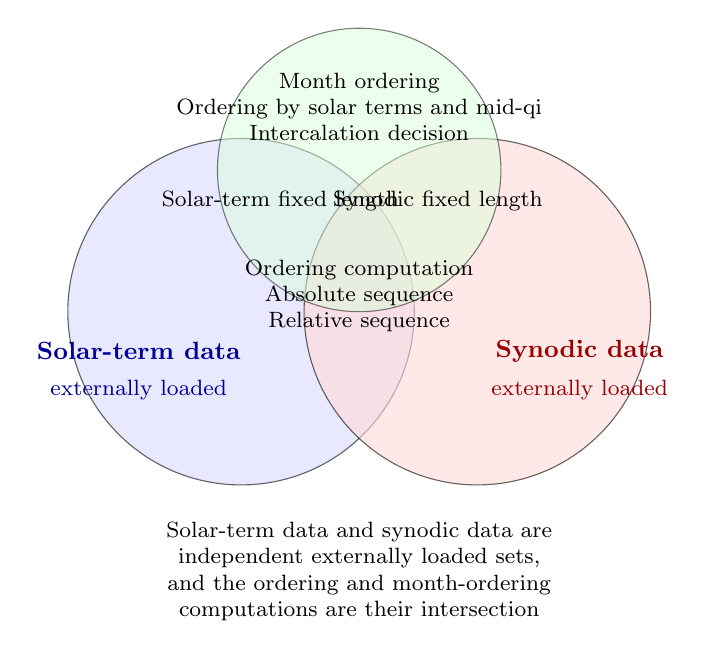
\begin{tikzpicture}[>=stealth]
        \draw[fill=blue!15, opacity=0.6] (-1.5, 0) circle (2.2cm);
        \draw[fill=red!15, opacity=0.6] (1.5, 0) circle (2.2cm);
        \draw[fill=green!15, opacity=0.5] (0, 1.8) circle (1.8cm);
        
        \node[font=\small\bfseries, blue!60!black] at (-2.8, -0.5) {Solar-term data};
        \node[font=\footnotesize, blue!60!black] at (-2.8, -1.0) {externally loaded};
        \node[font=\small\bfseries, red!60!black] at (2.8, -0.5) {Synodic data};
        \node[font=\footnotesize, red!60!black] at (2.8, -1.0) {externally loaded};
        
        \node[font=\footnotesize, align=center] at (0, 0.2) {Ordering computation\\Absolute sequence\\Relative sequence};
        \node[font=\footnotesize, align=center] at (0, 2.6) {Month ordering\\Ordering by solar terms and mid-qi\\Intercalation decision};
        \node[font=\footnotesize, align=center] at (-1.0, 1.4) {Solar-term fixed length};
        \node[font=\footnotesize, align=center] at (1.0, 1.4) {Synodic fixed length};
        
        \node[font=\footnotesize, text width=6cm, align=center] at (0, -3.3) {Solar-term data and synodic data are independent externally loaded sets,\\and the ordering and month-ordering computations are their intersection};
    \end{tikzpicture}
    \caption{Venn diagram: set relationships among solar-term data, synodic data and computational logic.}
    \label{fig:venn_data}
\end{figure}

\subsection{UML class diagram: the Range class and the temporal-unit inheritance hierarchy}

\begin{figure}[htbp]
    \centering
    \adjustbox{max width=\textwidth}{%
    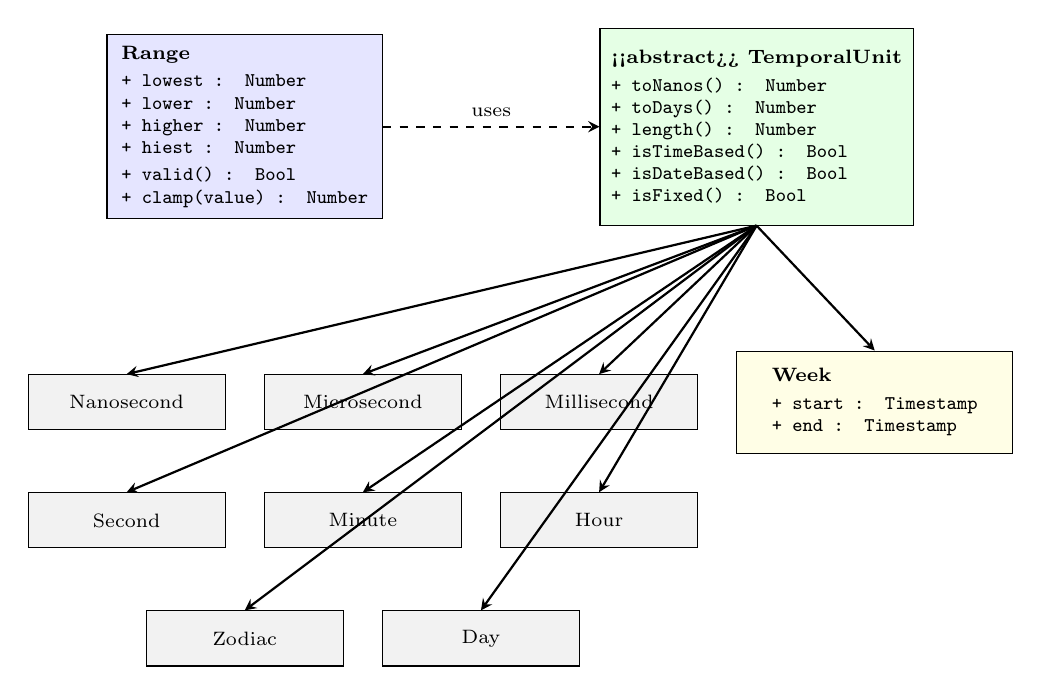
\begin{tikzpicture}[>=stealth,
        classbox/.style={draw, rectangle, minimum width=3.5cm, minimum height=2.0cm, align=left, font=\scriptsize, inner sep=4pt},
        subclassbox/.style={draw, rectangle, minimum width=2.5cm, minimum height=0.7cm, align=center, font=\scriptsize, inner sep=2pt},
        arrow/.style={->, thick, >=stealth}]
        
        \node[classbox, fill=blue!10] (range) at (0, 0) {
            \textbf{Range}\\[2pt]
            \texttt{+ lowest : Number}\\
            \texttt{+ lower : Number}\\
            \texttt{+ higher : Number}\\
            \texttt{+ hiest : Number}\\[2pt]
            \texttt{+ valid() : Bool}\\
            \texttt{+ clamp(value) : Number}
        };
        
        \node[classbox, fill=green!10, minimum height=2.5cm] (unit) at (6.5, 0) {
            \textbf{<<abstract>> TemporalUnit}\\[2pt]
            \texttt{+ toNanos() : Number}\\
            \texttt{+ toDays() : Number}\\
            \texttt{+ length() : Number}\\
            \texttt{+ isTimeBased() : Bool}\\
            \texttt{+ isDateBased() : Bool}\\
            \texttt{+ isFixed() : Bool}
        };
        
        \node[subclassbox, fill=gray!10] (ns) at (-1.5, -3.5) {Nanosecond};
        \node[subclassbox, fill=gray!10] (us) at (1.5, -3.5) {Microsecond};
        \node[subclassbox, fill=gray!10] (ms) at (4.5, -3.5) {Millisecond};
        \node[subclassbox, fill=gray!10] (sec) at (-1.5, -5) {Second};
        \node[subclassbox, fill=gray!10] (min) at (1.5, -5) {Minute};
        \node[subclassbox, fill=gray!10] (hr) at (4.5, -5) {Hour};
        \node[subclassbox, fill=gray!10] (zodiac) at (0, -6.5) {Zodiac};
        \node[subclassbox, fill=gray!10] (day) at (3, -6.5) {Day};
        \node[classbox, fill=yellow!10, minimum height=1.3cm] (week) at (8, -3.5) {
            \textbf{Week}\\[2pt]
            \texttt{+ start : Timestamp}\\
            \texttt{+ end : Timestamp}
        };
        
        \draw[->, thick, dashed] (range.east) -- node[above, font=\scriptsize] {uses} (unit.west);
        \draw[arrow] (unit.south) -- (ns.north);
        \draw[arrow] (unit.south) -- (us.north);
        \draw[arrow] (unit.south) -- (ms.north);
        \draw[arrow] (unit.south) -- (sec.north);
        \draw[arrow] (unit.south) -- (min.north);
        \draw[arrow] (unit.south) -- (hr.north);
        \draw[arrow] (unit.south) -- (zodiac.north);
        \draw[arrow] (unit.south) -- (day.north);
        \draw[arrow] (unit.south) -- (week.north);
    \end{tikzpicture}%
    }
    \caption{UML class diagram: the Range class and the TemporalUnit basic-unit inheritance hierarchy.}
    \label{fig:uml_basic_units}
\end{figure}

\begin{figure}[htbp]
    \centering
    \adjustbox{max height=0.8\textheight, max width=\textwidth}{%
    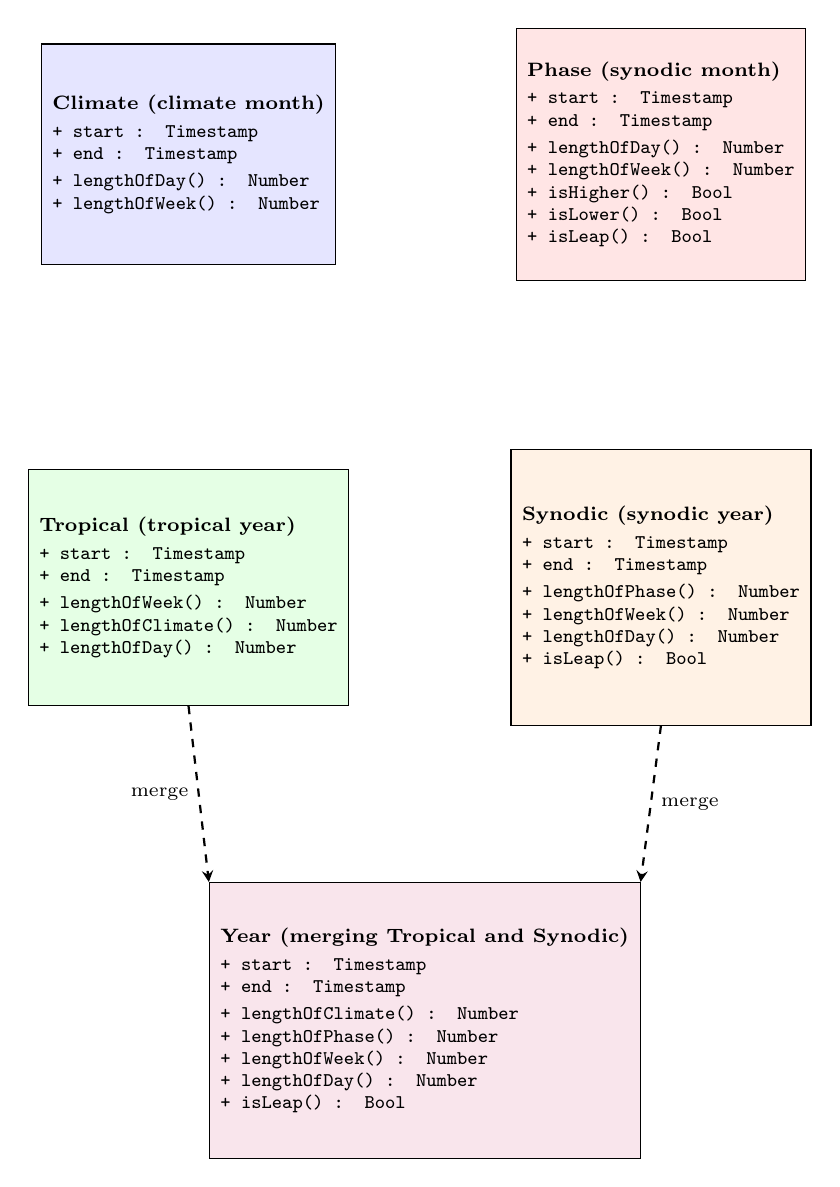
\begin{tikzpicture}[>=stealth,
        classbox/.style={draw, rectangle, minimum width=3.5cm, minimum height=2.8cm, align=left, font=\scriptsize, inner sep=4pt},
        arrow/.style={->, thick, >=stealth}]
        
        \node[classbox, fill=blue!10] (climate) at (-2.5, 0) {
            \textbf{Climate (climate month)}\\[2pt]
            \texttt{+ start : Timestamp}\\
            \texttt{+ end : Timestamp}\\[2pt]
            \texttt{+ lengthOfDay() : Number}\\
            \texttt{+ lengthOfWeek() : Number}
        };
        
        \node[classbox, fill=red!10, minimum height=3.2cm] (phase) at (3.5, 0) {
            \textbf{Phase (synodic month)}\\[2pt]
            \texttt{+ start : Timestamp}\\
            \texttt{+ end : Timestamp}\\[2pt]
            \texttt{+ lengthOfDay() : Number}\\
            \texttt{+ lengthOfWeek() : Number}\\
            \texttt{+ isHigher() : Bool}\\
            \texttt{+ isLower() : Bool}\\
            \texttt{+ isLeap() : Bool}
        };
        
        \node[classbox, fill=green!10, minimum height=3.0cm] (tropical) at (-2.5, -5.5) {
            \textbf{Tropical (tropical year)}\\[2pt]
            \texttt{+ start : Timestamp}\\
            \texttt{+ end : Timestamp}\\[2pt]
            \texttt{+ lengthOfWeek() : Number}\\
            \texttt{+ lengthOfClimate() : Number}\\
            \texttt{+ lengthOfDay() : Number}
        };
        
        \node[classbox, fill=orange!10, minimum height=3.5cm] (synodic) at (3.5, -5.5) {
            \textbf{Synodic (synodic year)}\\[2pt]
            \texttt{+ start : Timestamp}\\
            \texttt{+ end : Timestamp}\\[2pt]
            \texttt{+ lengthOfPhase() : Number}\\
            \texttt{+ lengthOfWeek() : Number}\\
            \texttt{+ lengthOfDay() : Number}\\
            \texttt{+ isLeap() : Bool}
        };
        
        \node[classbox, fill=purple!10, minimum height=3.5cm] (year) at (0.5, -11) {
            \textbf{Year (merging Tropical and Synodic)}\\[2pt]
            \texttt{+ start : Timestamp}\\
            \texttt{+ end : Timestamp}\\[2pt]
            \texttt{+ lengthOfClimate() : Number}\\
            \texttt{+ lengthOfPhase() : Number}\\
            \texttt{+ lengthOfWeek() : Number}\\
            \texttt{+ lengthOfDay() : Number}\\
            \texttt{+ isLeap() : Bool}
        };
        
        \draw[arrow, dashed, thick] (tropical.south) -- node[left, font=\scriptsize] {merge} (year.north west);
        \draw[arrow, dashed, thick] (synodic.south) -- node[right, font=\scriptsize] {merge} (year.north east);
    \end{tikzpicture}%
    }
    \caption{UML class diagram: the Climate, Phase, Tropical and Synodic classes and the merged Year class.}
    \label{fig:uml_complex_units}
\end{figure}

\subsection{UML class diagram: timestamps and temporal fields}

\begin{figure}[htbp]
    \centering
    \adjustbox{max width=\textwidth}{%
    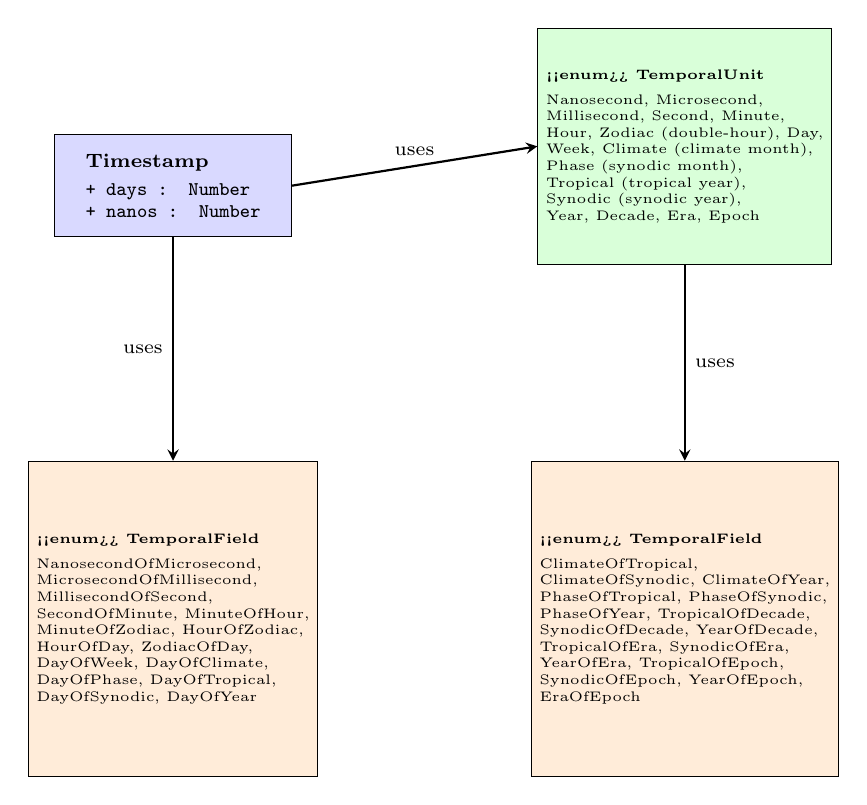
\begin{tikzpicture}[>=stealth,
        classbox/.style={draw, rectangle, minimum width=3.0cm, minimum height=1.3cm, align=left, font=\scriptsize, inner sep=4pt},
        enumbox/.style={draw, rectangle, minimum width=3.2cm, minimum height=2.0cm, align=left, font=\tiny, inner sep=3pt},
        arrow/.style={->, thick, >=stealth}]
        
        \node[classbox, fill=blue!15] (timestamp) at (0, 0) {
            \textbf{Timestamp}\\[2pt]
            \texttt{+ days : Number}\\
            \texttt{+ nanos : Number}
        };
        
        \node[enumbox, fill=green!15, minimum height=3.0cm] (unit) at (6.5, 0.5) {
            \textbf{<<enum>> TemporalUnit}\\[3pt]
            Nanosecond, Microsecond,\\
            Millisecond, Second, Minute,\\
            Hour, Zodiac (double-hour), Day,\\
            Week, Climate (climate month),\\
            Phase (synodic month),\\
            Tropical (tropical year),\\
            Synodic (synodic year),\\
            Year, Decade, Era, Epoch
        };
        
        \node[enumbox, fill=orange!15, minimum height=4.0cm] (field1) at (0, -5.5) {
            \textbf{<<enum>> TemporalField}\\[3pt]
            NanosecondOfMicrosecond,\\
            MicrosecondOfMillisecond,\\
            MillisecondOfSecond,\\
            SecondOfMinute, MinuteOfHour,\\
            MinuteOfZodiac, HourOfZodiac,\\
            HourOfDay, ZodiacOfDay,\\
            DayOfWeek, DayOfClimate,\\
            DayOfPhase, DayOfTropical,\\
            DayOfSynodic, DayOfYear
        };
        
        \node[enumbox, fill=orange!15, minimum height=4.0cm] (field2) at (6.5, -5.5) {
            \textbf{<<enum>> TemporalField}\\[3pt]
            ClimateOfTropical,\\
            ClimateOfSynodic, ClimateOfYear,\\
            PhaseOfTropical, PhaseOfSynodic,\\
            PhaseOfYear, TropicalOfDecade,\\
            SynodicOfDecade, YearOfDecade,\\
            TropicalOfEra, SynodicOfEra,\\
            YearOfEra, TropicalOfEpoch,\\
            SynodicOfEpoch, YearOfEpoch,\\
            EraOfEpoch
        };
        
        \draw[arrow] (timestamp.east) -- node[above, font=\scriptsize] {uses} (unit.west);
        \draw[arrow] (timestamp.south) -- node[left, font=\scriptsize] {uses} (field1.north);
        \draw[arrow] (unit.south) -- node[right, font=\scriptsize] {uses} (field2.north);
    \end{tikzpicture}%
    }
    \caption{UML class diagram: Timestamp and the TemporalUnit and TemporalField enumerations.}
    \label{fig:uml_timestamp}
\end{figure}

\begin{remark}[The calendrical meaning of the Range class]\label{rem:range_class}
The \textbf{Range} class defines a range constraint---\(lowest\le lower\le higher\le hiest\). \(valid()\) checks whether a value lies within \([lowest,hiest]\), and \(clamp(value)\) truncates a value to that range. In calendar systems the Range class is used to constrain the admissible value ranges of the various time fields---for example the relative sequence of months must lie within \([1,12]\), and the relative sequence of days must lie within \([1,30]\) (a long month) or \([1,29]\) (a short month).
\end{remark}

\begin{remark}[The lengthOfWeek method of Climate and Phase]\label{rem:climate_phase_length}
Both \textbf{Climate} (the climate month) and \textbf{Phase} (the synodic month) contain a \textbf{lengthOfWeek} method---it returns the number of whole weeks within the month. The length of a climate month lies within the range \(14\)--\(18\) days and the length of a synodic month is about \(29.53\) days. Hence a climate month usually contains \(2\)--\(3\) whole weeks and a synodic month usually contains \(4\)--\(5\) whole weeks. The lengthOfWeek method is of practical significance for arranging work schedules within a month and for determining the lunar-calendar date corresponding to each day of the week.
\end{remark}

\begin{remark}[The length method of TemporalUnit and isFixed]\label{rem:temporal_unit_length}
\textbf{length()} returns the number of units of the next lower level contained in the current unit: \(\texttt{Day.length()}=24\), \(\texttt{Week.length()}=7\), \(\texttt{Climate.length()}\approx 15\) (within the range \(14\)--\(18\) days), \(\texttt{Phase.length()}\approx 29.53\), \(\texttt{Tropical.length()}=12\), \(\texttt{Synodic.length()}=12\) or \(13\). \textbf{isFixed} returns whether the unit has a fixed length: \(\texttt{Hour.isFixed()}=true\), \(\texttt{Phase.isFixed()}=false\), \(\texttt{Climate.isFixed()}=false\).
\end{remark}

\begin{remark}[The merge semantics of the Year class]\label{rem:year_class}
\textbf{Year} is the merge of \textbf{Tropical} and \textbf{Synodic}---it possesses at once \(\texttt{lengthOfClimate}\) (the number of climate months in the tropical year \(=12\)), \(\texttt{lengthOfPhase}\) (the number of synodic months in the year \(=12\) or \(13\)), \(\texttt{lengthOfWeek}\) (the number of weeks in the year), \(\texttt{lengthOfDay}\) (the number of days in the year \(=365\) or \(366\)) and \(\texttt{isLeap}\) (the leap-year decision). The merge embodies the essence of the lunisolar calendar---a calendar year is described simultaneously by two systems, the solar calendar (climate months) and the lunar calendar (synodic months).
\end{remark}

\subsection{Flowchart}

\begin{figure}[htbp]
    \centering
    \adjustbox{max width=\textwidth}{%
    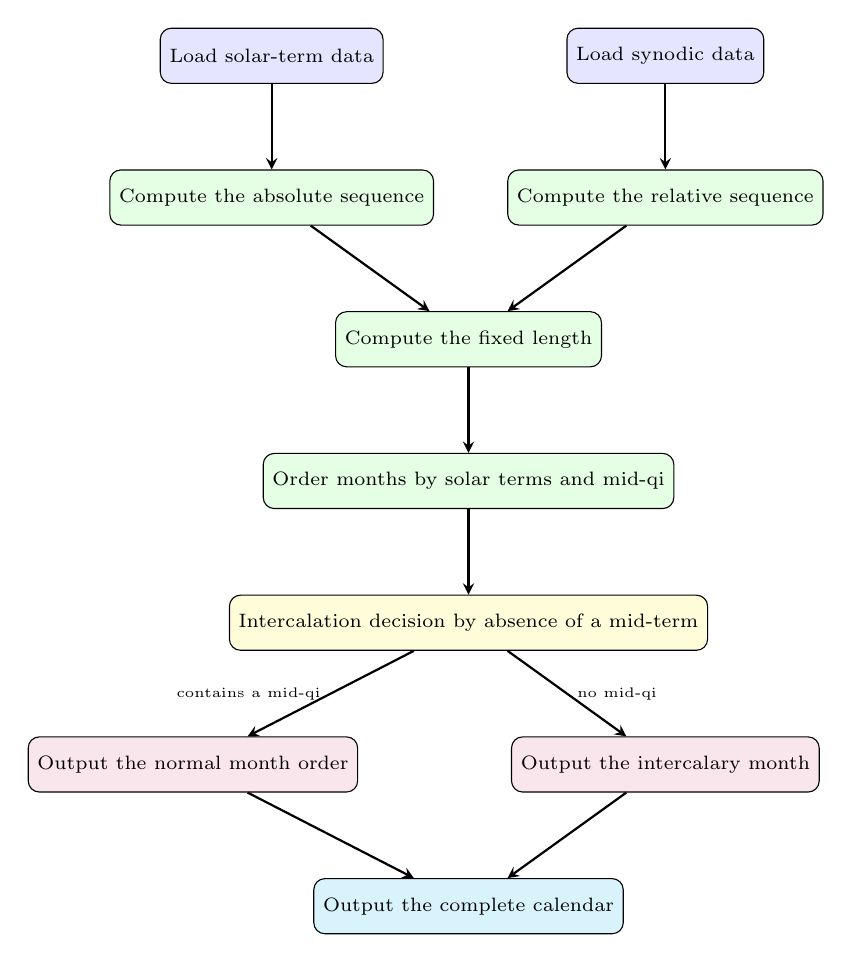
\begin{tikzpicture}[>=stealth,
        databox/.style={draw, rounded corners, fill=blue!10, minimum width=2.2cm, minimum height=0.7cm, align=center, font=\scriptsize},
        calcbox/.style={draw, rounded corners, fill=green!10, minimum width=2.2cm, minimum height=0.7cm, align=center, font=\scriptsize},
        outbox/.style={draw, rounded corners, fill=purple!10, minimum width=2.2cm, minimum height=0.7cm, align=center, font=\scriptsize},
        arrow/.style={->, thick, >=stealth}]
        
        \node[databox] (load_jieqi) at (0, 0) {Load solar-term data};
        \node[databox] (load_shuo) at (5, 0) {Load synodic data};
        \node[calcbox] (calc_abs) at (0, -1.8) {Compute the absolute sequence};
        \node[calcbox] (calc_rel) at (5, -1.8) {Compute the relative sequence};
        \node[calcbox] (calc_len) at (2.5, -3.6) {Compute the fixed length};
        \node[calcbox] (dingyue) at (2.5, -5.4) {Order months by solar terms and mid-qi};
        \node[calcbox, fill=yellow!15] (run_check) at (2.5, -7.2) {Intercalation decision by absence of a mid-term};
        \node[outbox] (out_normal) at (-1, -9) {Output the normal month order};
        \node[outbox] (out_run) at (5, -9) {Output the intercalary month};
        \node[outbox, fill=cyan!15] (out_calendar) at (2.5, -10.8) {Output the complete calendar};
        
        \draw[arrow] (load_jieqi) -- (calc_abs);
        \draw[arrow] (load_shuo) -- (calc_rel);
        \draw[arrow] (calc_abs) -- (calc_len);
        \draw[arrow] (calc_rel) -- (calc_len);
        \draw[arrow] (calc_len) -- (dingyue);
        \draw[arrow] (dingyue) -- (run_check);
        \draw[arrow] (run_check) -- node[left, font=\tiny] {contains a mid-qi} (out_normal);
        \draw[arrow] (run_check) -- node[right, font=\tiny] {no mid-qi} (out_run);
        \draw[arrow] (out_normal) -- (out_calendar);
        \draw[arrow] (out_run) -- (out_calendar);
    \end{tikzpicture}%
    }
    \caption{Calendar computation flowchart: external data loading$\to$ordering$\to$fixed length$\to$ordering of months by solar terms and mid-qi$\to$intercalation decision$\to$calendar output.}
    \label{fig:flow_calendar}
\end{figure}

\section{The independence of the solar-term system and the synodic-month system}
\label{sec:calendar_independence}

\subsection{The solar-term system---the solar calendar}

\begin{definition}[Solar-term system]\label{def:solar_term_system}
The \textbf{twenty-four solar terms} are a solar-calendar system originating in ancient China, which divides the tropical year equally into \(24\) time nodes. The solar-term system takes the tropical year \(T_{\text{trop}}\) as its basic period.
\end{definition}

\begin{definition}[Mean solar-term method]\label{def:pingqi_method}
The \textbf{mean solar-term method} divides the tropical year uniformly into \(24\) parts: \(\Delta T_{\text{pingqi}}=T_{\text{trop}}/24\approx 15.2184\) days. It corresponds to mean solar time---a uniform division of time.
\end{definition}

\begin{definition}[True solar-term method]\label{def:dingqi_method}
The \textbf{true solar-term method} determines the instants of the solar terms from the actual apparent position of the Sun on the ecliptic, placing one solar term every \(15^\circ\). It corresponds to true solar time---a non-uniform division of time.
\end{definition}

\begin{proposition}[Comparison of the mean and true solar-term methods]\label{prop:pingqi_dingqi_comparison}
The mean solar-term method is based on a uniform division of time (corresponding to mean solar time), whilst the true solar-term method is based on a uniform angular division of the solar ecliptic longitude (corresponding to true solar time). The transition from the mean to the true solar-term method is a transition from the uniformisation of time to the uniformisation of ecliptic longitude.
\end{proposition}

\begin{proof}
By \cref{def:pingqi_method}, the mean solar-term method divides the tropical year uniformly into \(24\) parts, and the solar-term interval \(\Delta T_{\text{pingqi}}=T_{\text{trop}}/24\) is constant, that is, a uniform division of the time axis. By \cref{def:dingqi_method}, the true solar-term method takes a solar term every \(15^\circ\) of solar ecliptic longitude; since the apparent motion of the Sun is fast at perihelion (near the winter solstice) and slow at aphelion (near the summer solstice), the time intervals between the solar terms are non-uniform, corresponding to a uniform angular division of the ecliptic. Hence the mean solar-term method achieves the uniformisation of time and the true solar-term method achieves the uniformisation of ecliptic longitude.
\end{proof}

\subsection{The synodic-month system---the lunar calendar}

\begin{definition}[Synodic-month system]\label{def:synodic_month_system}
The \textbf{synodic-month system} is a lunar-calendar system based on the synodic period of the Moon's revolution about the Earth. \(T_{\text{syn}}=29.5305889\) mean solar days. Twelve synodic months constitute a lunar year, which is shorter than the tropical year by about \(10.875\) days.
\end{definition}

\begin{proposition}[The independent period of the synodic-month system]\label{prop:synodic_month_conservation}
The periods of the synodic-month system and the solar-term system are incommensurable, that is,
\[
\frac{T_{\text{trop}}}{T_{\text{syn}}}\approx 12.36827,
\]
hence it is impossible to unify the solar calendar and the lunar calendar perfectly by a simple integer ratio.
\end{proposition}

\begin{proof}
By \cref{def:synodic_month_system}, the synodic-month system has period \(T_{\text{syn}}=29.5305889\) mean solar days; by \cref{def:fixed_length}, the solar-term system has period \(T_{\text{trop}}=365.2421897\) mean solar days. Their ratio
\[
\frac{T_{\text{trop}}}{T_{\text{syn}}}=\frac{365.2421897}{29.5305889}\approx 12.36827
\]
agrees with no \(p/q\) of bounded denominator within the current precision of measurement (an \textbf{empirical observation / research programme}; see \cref{prop:length_incommensurability}), so there exist no integers \(p,q\) such that \(p\,T_{\text{trop}}=q\,T_{\text{syn}}\). Hence the period of the synodic-month system is independent of the period of the solar-term system, and each preserves its own period scale.
\end{proof}

\subsection{Coordination of the lunisolar calendar---intercalation}

\begin{lemma}[Metonic cycle (seven intercalary months in nineteen years)]\label{ch18_metonic_cycle}
Nineteen tropical years and \(235\) synodic months are approximately equal in length:
\[
19\,T_{\text{trop}}\approx 235\,T_{\text{syn}},
\]
where \(19\,T_{\text{trop}}\approx 6939.60\) days and \(235\,T_{\text{syn}}\approx 6939.69\) days, the two differing by about \(0.09\) days. Hence after \(19\) years the phases of the Sun and the Moon are almost restored; moreover \(235=12\times 19+7\), so \(7\) intercalary months must be inserted within \(19\) years (the intercalation period ratio being \(235/19\)).
\end{lemma}

\begin{proof}
From the fixed-length values of \cref{def:fixed_length} we compute
\[
19\,T_{\text{trop}}=19\times 365.2421897=6939.6016\ \text{days},
\]
\[
235\,T_{\text{syn}}=235\times 29.5305889=6939.6884\ \text{days}.
\]
The two differ by
\[
6939.6884-6939.6016=0.0868\ \text{days},
\]
which is far smaller than one synodic month (\(29.53\) days); hence \(19\) tropical years and \(235\) synodic months are restored almost simultaneously, and the phases of the solar calendar and the lunar calendar close within \(19\) years.
Without intercalation, \(19\) years would contain only \(12\times 19=228\) synodic months, \(7\) fewer than \(235\). Hence \(7\) intercalary months must be added within \(19\) years so that the two calendars align, which gives the intercalation period ratio
\[
\frac{235}{19}.
\qedhere
\]
\end{proof}

\begin{definition}[Intercalation---phase alignment of the two systems]\label{def:intercalation}
Seven intercalary months in nineteen years (the Metonic cycle): \(19\times T_{\text{trop}}\approx 6939.60\) days, \(235\times T_{\text{syn}}\approx 6939.69\) days. After \(19\) years the phases of the Sun and the Moon are almost restored. The intercalation period ratio is \(235/19\).
\end{definition}

\begin{proposition}[Intercalation by absence of a mid-term---consistency with ordering months by solar terms and mid-qi]\label{prop:wuzhongqi_rule}
If within a synodic month there is only a solar term and no mid-qi, then that month is an intercalary month---this agrees with the criterion of \cref{prop:wuzhongqi_run}. Intercalation by absence of a mid-term ensures that the beginning of the year (the first month) always lies around Lichun.
\end{proposition}

\begin{proof}
The first sentence is the criterion for an intercalary month of \cref{prop:wuzhongqi_run}, whose mechanism was given in the proof of that proposition (a month without a mid-qi occurs when the interval between adjacent mid-qi exceeds the fixed length of the synodic month). The second sentence explains the purpose of intercalation: by \cref{def:jieqi_zhongqi_dingyue}, the synodic month containing Lichun and Yushui is the first month (the Tiger month); intercalation by absence of a mid-term guarantees that the first month always contains Lichun, so that the deviation of the beginning of the year from Lichun does not exceed the order of one synodic month, and the beginning of the year therefore always lies around Lichun.
\end{proof}

\subsection{Algorithm 1: continued-fraction intercalation}
\label{subsec:continued_fraction_intercalation_algorithm}

Algorithm 1 is the \textbf{number-theoretic/mean} route: it uses only the mean period ratio
\[
\rho=\frac{T_{\text{trop}}}{T_{\text{syn}}},
\]
and reads no specific new-moon or mid-qi instant. Its input is \(\rho\) together with a window or tolerance; its output is an intercalation sequence (or a count per window), not `which specific month is intercalary'.

\begin{enumerate}[label=\textbf{Step \arabic*.}, leftmargin=*]
    \item Compute the continued-fraction convergents \(p_j/q_j\) of \(\rho\) (\cref{thm:calendar_continued_fraction_best}).
    \item Choose the smallest window \(q_j\) with \(1/q_{j+1}<\varepsilon\), or take a prescribed window \(M\).
    \item Generate the balanced intercalation sequence
    \[
    N_m=\operatorname{round}((m+1)\rho)-\operatorname{round}(m\rho),
    \qquad m=0,\dots,M-1,
    \]
    or use upper/lower intercalation (\cref{thm:calendar_intercalation_error_bound}).
    \item Output the intercalary positions/count and the cumulative error
    \[
    E_M=\sum_{m=0}^{M-1}N_m-M\rho.
    \]
\end{enumerate}

\textbf{Guarantee}: at a convergent window \(M=q_j\), \(|E_M|<1/q_{j+1}\) (\cref{thm:calendar_continued_fraction_best}); balanced intercalation has \(|E_M|\le1/2\) for every \(M\) (\cref{thm:calendar_intercalation_error_bound}). For \(\rho=12.36827\), \(q=19,p=235\): seven intercalary months in nineteen years, \(\delta_{19}=0.00295\).

\textbf{Complexity}: \(O(\log M)\) for the continued fraction and \(O(M)\) for the sequence.

\textbf{Limitation}: Algorithm 1 gives a count/mean rhythm, not a specific month; to obtain a month one still needs a convention mapping the sequence to month positions. Algorithm 2 solves that problem, but it is not a discretisation of Algorithm 1: it is an independent second route.

\subsection{Algorithm 2: exact event-driven intercalation}
\label{subsec:exact_intercalation_algorithm}

Algorithm 2 is the \textbf{event/astronomical} route, independent of Algorithm 1: it uses neither \(\rho\), nor continued-fraction convergents, nor mean periods; it uses only the exact new-moon sequence \(n_i\) and mid-qi sequence \(z_j\). Its input is the two event sequences and its output is the specific intercalary month. The definitions, proposition and validation tables below give the full specification of Algorithm 2.

\textbf{Exact month intervals and mid-qi counts.}

\begin{definition}[Exact month intervals and mid-qi counts]
\label{def:exact_month_term_count}
Let \(n_i\) be the Julian day number of the \(i\)-th new moon and \(z_j\) that of the \(j\)-th mid-qi. Take the day boundary of the new-moon day, \(s_i=\lfloor n_i\rfloor\), as the beginning of the month:
\[
s_i=\lfloor n_i\rfloor,\qquad I_i=[s_i,s_{i+1}).
\]
Call
\[
c_i=\#\{j: s_i\le z_j<s_{i+1}\}
\]
the \textbf{mid-qi count} of the \(i\)-th synodic month.
\end{definition}

\begin{remark}[The day-boundary convention]
\label{rem:exact_day_boundary}
A traditional calendar begins the month on the day of the new moon, not at the exact instant of the new moon. If the exact instant \(n_i\) is used as the month boundary, a mid-qi falling within a few hours of the new moon is assigned to the neighbouring month, which produces many boundary errors. With \(s_i=\lfloor n_i\rfloor\) the decision agrees with the calendar labels. Table \ref{tab:exact_intercalation_comparison} gives the quantitative comparison: on the same worksheet, the exact-instant per-month rule has \(272\) mismatches, the day-boundary per-month rule \(48\), and the day-boundary plus year-boundary rule \(0\).
\end{remark}

\textbf{Winter-solstice years.}

\begin{definition}[Winter-solstice year and mid-qi count]
\label{def:winter_solstice_year}
Let \(w_y\) be the Julian day number of the \(y\)-th winter solstice and \(m_y\) the index of the synodic month containing \(w_y\):
\[
s_{m_y}\le w_y<s_{m_y+1}.
\]
Call
\[
Y_y=\{m_y,m_y+1,\dots,m_{y+1}-1\}
\]
the \(y\)-th \textbf{winter-solstice year}, and write
\[
C_y=\#\{j: w_y\le z_j<w_{y+1}\}.
\]
\end{definition}

\textbf{The exact decision.}

\begin{definition}[Exact intercalation by absence of a mid-term]
\label{def:exact_wuzhongqi_decision}
For the \(y\)-th winter-solstice year:
\begin{enumerate}[label=(\roman*)]
    \item if \(|Y_y|=12\), the year has no intercalary month;
    \item if \(|Y_y|=13\), the first month in \(Y_y\) with \(c_i=0\) is intercalary;
    \item if \(|Y_y|\notin\{12,13\}\) or \(C_y\ne12\), flag the year for review and do not decide.
\end{enumerate}
\end{definition}

\begin{proposition}[Structure of the exact decision]
\label{prop:exact_wuzhongqi_consistency}
Under the day-boundary convention, if \(C_y=12\), then:
\begin{enumerate}[label=(\roman*)]
    \item if \(|Y_y|=13\), at least one month satisfies \(c_i=0\);
    \item if \(|Y_y|=12\), the year has no intercalary month;
    \item hence `a 13-month year takes the first month without a mid-qi, while a 12-month year has none' is consistent with the rule of intercalation by absence of a mid-term.
\end{enumerate}
\end{proposition}

\begin{proof}
(i) By the pigeonhole principle, \(12\) mid-qi placed in \(13\) months leave at least one month without a mid-qi. (ii) An intercalary month occurs only in a 13-month year; this is the year-length convention of intercalation by absence of a mid-term, and a 12-month year has no intercalary month. (iii) follows directly from (i) and (ii).
\end{proof}

\begin{remark}[Principal mid-qi and secondary solar-term/mid-qi: a column that must be read]
\label{rem:main_secondary_terms}
Each monthly record of the \textit{Shouxing} compilation contains three solar-term columns: \textbf{principal solar term}, \textbf{principal mid-qi} and \textbf{secondary solar-term/mid-qi}. When a synodic month contains two solar terms or two mid-qi, the second is recorded in the secondary column. If only the principal mid-qi column is read, a month containing two mid-qi loses one, so the winter-solstice year has only \(11\) or \(10\) mid-qi and a normal month is misclassified as intercalary. Reading the secondary column as well, and retaining only the twelve mid-qi names, restores \(12\) mid-qi per winter-solstice year; all \(290{,}654\) months then agree with the labels. This is not a data error but a question of completeness of the data model.
\end{remark}

\textbf{The algorithm.}

\begin{enumerate}[label=\textbf{Step \arabic*.}, leftmargin=*]
    \item Read the new moons \(n_i\), the month-name labels, the principal mid-qi (columns \(9/10\)) and the secondary solar-term/mid-qi (columns \(11/12\)) from every worksheet; keep only the twelve mid-qi names and deduplicate by Julian day number.
    \item Set \(s_i=\lfloor n_i\rfloor\) and assign each mid-qi to its month by binary search:
    \[
    k_j=\max\{k: s_k\le z_j\},
    \]
    obtaining \(c_i=\#\{j:k_j=i\}\).
    \item Take the winter solstices \(w_y\), locate \(m_y\), and form the winter-solstice years \(Y_y\).
    \item If \(|Y_y|=13\), mark the first month in \(Y_y\) with \(c_i=0\) as intercalary; if \(|Y_y|=12\), mark none.
    \item Compare with the `run' (intercalary) label in the month name; output mismatching months and years flagged for review.
\end{enumerate}

Complexity: sorting \(O(N\log N)\), assignment \(O((N+M)\log N)\), year boundaries \(O(N)\); with \(N=290{,}654\) and \(M=282{,}000\), this takes seconds on an ordinary machine (apart from parsing the workbook).

\begin{table}[htbp]
\centering
\caption{Validation of the exact intercalation algorithm on the \textit{Shouxing} compilation (24 worksheets).}
\label{tab:exact_intercalation_validation}
\begin{tabular}{lr}
\toprule
Item & Value \\
\midrule
Synodic months & \(290{,}654\) \\
Principal/secondary mid-qi records (including boundary duplicates) & \(282{,}000\) \\
Intercalary-month labels & \(8{,}654\) \\
Winter-solstice years & \(23{,}499\) \\
of which 12-month years & \(14{,}845\) \\
of which 13-month years & \(8{,}654\) \\
Months without mid-qi in 13-month years & \(8{,}654\) (one per year) \\
Predicted intercalary months & \(8{,}654\) \\
Mismatches & \(0\) \\
\bottomrule
\end{tabular}
\end{table}

\begin{table}[htbp]
\centering
\caption{Stepwise improvement on the first worksheet (\(12{,}368\) months); all three rows read the principal mid-qi column only. The first two rows use no year boundary; the third uses the winter-solstice year. The all-table result after also reading the secondary column is Table \ref{tab:exact_intercalation_validation}.}
\label{tab:exact_intercalation_comparison}
\begin{tabular}{@{}p{9.6cm}r@{}}
\toprule
Method & Mismatches \\
\midrule
Exact instants, per-month absence of a mid-qi & \(272\) \\
Day boundary, per-month absence of a mid-qi & \(48\) \\
Day boundary \(+\) winter-solstice year, first month without a mid-qi & \(0\) \\
\bottomrule
\end{tabular}
\end{table}

On the full table, the day-boundary plus winter-solstice-year rule with the principal mid-qi column alone still has \(160\) false positives; reading the secondary column reduces this to \(0\). All \(160\) false positives come from months that contain two mid-qi, the second recorded in the secondary column; once that column is read, every winter-solstice year is restored to \(12\) mid-qi and the false positives disappear.

\begin{remark}[Relation to the mean period density]
\label{rem:exact_vs_mean_density}
The mean model replaces the month length and the mid-qi interval by \(T_{\text{syn}}\) and \(T_{\text{trop}}/12\), and gives the \textbf{mean rhythm} of one intercalary month every \(2.715\) years, or seven in nineteen years. With exact data the local density should be written as
\[
D(t)=\frac{1}{L_m(t)}-\frac{1}{L_z(t)},
\]
where \(L_m^{(i)}=n_{i+1}-n_i\) and \(L_z^{(j)}=z_{j+1}-z_j\) are the exact local intervals. This is a calendar instance of the frequency-difference density \(\Delta_{f,g}\) in \cref{def:dyn_period_difference_density} (with \(f\) the mid-qi interval and \(g\) the synodic month); multiplying it by the interval normalisation factor \((b-a)/(N_fN_g)\) (which becomes \(T_f-T_g\) on the beat period) gives the period-difference density \(D_{f,g}\), whose integral over one beat is the time difference. Hence
\[
\int_{s_i}^{s_{i+1}}D(t)\,dt
=1-\frac{L_m^{(i)}}{L_z^{(i)}}.
\]
\(D(t)\) is an explanatory quantity: it shows why a month `swallows' or `loses' a mid-qi; but the \textbf{decision} for an intercalary month uses the event count \(c_i\), not a density threshold. The mean density remains a tool for the long-term average and for prediction.
\end{remark}

\begin{remark}[Relation to the discrete-sampling chapter]
\label{rem:exact_intercalation_sampling}
Seven intercalary months in nineteen years is the continued-fraction approximation to \(\rho=T_{\text{trop}}/T_{\text{syn}}\) (\cref{ch18_metonic_cycle}, \cref{thm:calendar_continued_fraction_best}), but Algorithm 2 is not a discretisation of that approximation: it executes the event rule of intercalation by absence of a mid-term directly, without passing through \(\rho\) or continued fractions. \cref{thm:calendar_sampling_unification_parallel} identifies calendar intercalation and sampling intercalation as the same mathematical object; Algorithm 2 is the independent realisation of that isomorphism at the level of new-moon and mid-qi events: the intercalary-month decision is equivalent to a discrete check of congruence-angle closure.
\end{remark}

\begin{remark}[Scope of the validation]
\label{rem:exact_intercalation_scope}
The zero mismatch is an \textbf{empirical validation} on the \textit{Shouxing} compilation, not a theorem about every calendar. Historical calendar reforms, time-zone conventions, ephemeris accuracy and the definition of the day boundary may change the attribution of individual months; when changing the data set, calibrate the day boundary and the mid-qi table before running the algorithm. The algorithm itself depends only on `event sequence \(+\) winter-solstice year \(+\) mid-qi count', not on mean periods.
\end{remark}

\subsection{Independence and comparison of the two algorithms}
\label{subsec:two_intercalation_algorithms_comparison}

Algorithms 1 and 2 are two independent routes, not approximations or special cases of one another:

\begin{itemize}
    \item Algorithm 1 takes the mean period ratio \(\rho\) as input, uses continued-fraction convergents and a balanced sequence, and outputs a count/mean rhythm; it knows nothing about specific new moons or mid-qi.
    \item Algorithm 2 takes the exact event sequences as input, uses the winter-solstice year and mid-qi counts, and outputs the specific intercalary month; it uses neither \(\rho\) nor continued fractions.
\end{itemize}

They can cross-check each other: Algorithm 1 gives the long-term count (for example seven in nineteen years), Algorithm 2 gives the specific month; with complete data, the mean rhythm of Algorithm 1 should agree with the statistics of Algorithm 2. The Metonic example is a \textbf{consistency check} of the two, not a derivation of Algorithm 2.

\begin{table}[htbp]
\centering
\small
\caption{Comparison of the two intercalation algorithms.}
\label{tab:two_intercalation_algorithms}
\begin{tabular}{@{}>{\raggedright\arraybackslash}p{2.6cm}>{\raggedright\arraybackslash}p{4.9cm}>{\raggedright\arraybackslash}p{4.9cm}@{}}
\toprule
Item & Algorithm 1: continued fraction & Algorithm 2: exact events \\
\midrule
Input & \(\rho=T_{\text{trop}}/T_{\text{syn}}\), window/tolerance & new-moon \(n_i\) and mid-qi \(z_j\) event sequences \\
Core & continued-fraction convergents, balanced sequence & winter-solstice year, first month without mid-qi \\
Output & intercalation sequence/count & specific intercalary month \\
Dependence & mean period ratio & exact events, day boundary \\
Accuracy & \(|E_M|<1/q_{j+1}\) (convergent window) & zero mismatch for complete data \\
Complexity & \(O(\log M+M)\) & \(O((N+M)\log N)\) \\
\bottomrule
\end{tabular}
\end{table}

\begin{remark}[Independence]
\label{rem:two_algorithms_independent}
Algorithm 2 is not an `implementation' of Algorithm 1 on finite data: the continued-fraction convergents, the windows \(q_j\) and the period ratio \(\rho\) of Algorithm 1 appear neither in the input nor in the steps of Algorithm 2; the winter-solstice year, the mid-qi counts and the day boundary of Algorithm 2 appear nowhere in Algorithm 1. The two meet only at the calendar rule of `intercalation by absence of a mid-term': Algorithm 1 approximates that rule through the mean period ratio, while Algorithm 2 executes it exactly through event counts. Algorithm 2 can therefore stand as a second algorithm independent of continued-fraction intercalation, for exact data; Algorithm 1 remains the tool for mean rhythm, window selection and prediction.
\end{remark}

\section{The periodic structure of the lunisolar calendar}
\label{sec:lunisolar_structure}

\begin{theorem}[The three periodic scales of the lunisolar calendar]\label{thm:lunisolar_grammar_unity}
\begin{enumerate}[label=(\roman*)]
    \item \textbf{Solar-term system (solar calendar)}: with the tropical year \(T_{\text{trop}}\) as period, the distribution of the solar terms within the year being determined by the solar ecliptic longitude.
    \item \textbf{Synodic-month system (lunar calendar)}: with the synodic month \(T_{\text{syn}}\) as period, the repetition of the lunar phases being determined by the relative positions of the Sun, the Earth and the Moon.
    \item \textbf{Intercalation system (coordination layer)}: with seven intercalary months in nineteen years as its rule and the intercalation period ratio \(235/19\), coordinating the first two sets of periods on the scale of \(19\) years.
\end{enumerate}
\end{theorem}

\begin{proof}
The realisation of the three periodic scales is verified item by item:
\begin{enumerate}[label=(\roman*)]
\item the solar-term system has the tropical year \(T_{\text{trop}}\) as period (\cref{def:solar_term_system}), and the mean solar-term method divides it uniformly into \(24\) parts (\cref{def:pingqi_method}), giving a uniform division of the solar terms on the time axis.
\item the synodic-month system has \(T_{\text{syn}}\) as period (\cref{def:synodic_month_system}) and measures the synodic phase of the Moon's revolution about the Earth---the repetition period of the lunar phases.
\item the intercalation system coordinates the first two: by the Metonic-cycle lemma (seven intercalary months in nineteen years), \(235\) synodic months are arranged within \(19\) tropical years, with intercalation period ratio \(235/19\); this is the coordination layer between the two independent periods.
\end{enumerate}
\end{proof}

\section{The mathematical structure of astronomical and historical year numbering}
\label{sec:calendar_year_numbering}

\begin{definition}[Astronomical year numbering]\label{def:astronomical_year_numbering}
Astronomical year numbering is continuous on the integer axis: the year \(1\) CE is \(+1\), the year \(1\) BCE is \(0\), and the year \(n\) BCE is \(-(n-1)\). \(0\) is a legitimate year number.
\end{definition}

\begin{definition}[Historical year numbering]\label{def:historical_year_numbering}
In historical year numbering there is no year \(0\) CE---the year \(1\) BCE is followed directly by the year \(1\) CE.
\end{definition}

\begin{proposition}[Conversion between astronomical and historical year numbering]\label{prop:year_conversion}
When \(Y_{\text{ast}}\ge 1\), \(Y_{\text{hist}}=Y_{\text{ast}}\); when \(Y_{\text{ast}}\le 0\), \(Y_{\text{hist}}=1-Y_{\text{ast}}\).
\end{proposition}

\begin{proof}
By \cref{def:astronomical_year_numbering}, astronomical year numbering writes the year \(1\) CE as \(+1\) and the year \(n\) BCE as \(-(n-1)\). When \(Y_{\text{ast}}\ge 1\), astronomical and historical year numbering give the same CE year number, so \(Y_{\text{hist}}=Y_{\text{ast}}\). When \(Y_{\text{ast}}\le 0\), \(Y_{\text{ast}}\) corresponds to the year \((1-Y_{\text{ast}})\) BCE: for example \(Y_{\text{ast}}=0\) corresponds to the year \(1\) BCE and \(Y_{\text{ast}}=-1\) to the year \(2\) BCE; in general, solving \(-(n-1)=Y_{\text{ast}}\) gives \(n=1-Y_{\text{ast}}\), hence \(Y_{\text{hist}}=1-Y_{\text{ast}}\).
\end{proof}

\begin{theorem}[Correction theorem for time intervals crossing the Common Era boundary]\label{thm:cross_era_correction}
Starting from the year \(m\) BCE and passing through \(P\) years, the resulting historical year is:
\[
Y_{\text{hist}}=\begin{cases}
m-P, & P<m,\\
P-m+1, & P\ge m.
\end{cases}
\]
When \(P\ge m\) (crossing the Common Era boundary), a \(+1\) correction is required.
\end{theorem}

\begin{proof}
Compute in the astronomical-year-numbering coordinates of \cref{prop:year_conversion}. The astronomical year number of the year \(m\) BCE is \(Y_{\text{ast}}=-(m-1)\) (\cref{def:astronomical_year_numbering}); after \(P\) years the astronomical year number becomes \(Y'_{\text{ast}}=-(m-1)+P=P-m+1\).
\begin{itemize}
\item If \(P<m\), then \(Y'_{\text{ast}}=P-m+1\le 0\), which is still BCE; by \cref{prop:year_conversion}, \(Y_{\text{hist}}=1-Y'_{\text{ast}}=m-P\).
\item If \(P\ge m\), then \(Y'_{\text{ast}}=P-m+1\ge 1\), which has entered the Common Era; here \(Y_{\text{hist}}=Y'_{\text{ast}}=P-m+1\), where the \(+1\) is precisely the correction required for crossing the boundary `there is no year \(0\) CE'.
\end{itemize}
Combining the two cases gives the assertion.
\end{proof}

\section{The epoch system of the *Huainanzi*, `Tianwenxun'}
\label{sec:huainanzi}

\begin{definition}[One Ji]\label{def:yiji}
One Ji is \(76\) years: \(76\times 365.25=940\times 29.53085=27759\) days---the least common multiple period of the tropical year and the synodic month.
\end{definition}

\begin{definition}[One Bu---the Great Conclusion after 1520 years]\label{def:yibu}
One Bu is \(1520\) years \(=76\times 20\). \(1520\bmod 60=20\)---on passing through one Bu, the sexagenary cycle advances by \(20\) places.
\end{definition}

\begin{theorem}[Theorem on the sexagenary shift over one Bu]\label{thm:yibu_ganzhi_shift}
After \(k\) Bu the sexagenary index is \(S_k=S_0+20k\pmod{60}\). For \(k=3\) the sexagenary sign is restored. Within one Bu the sexagenary sign advances by \(+20\), cycling through the three pillars Jiayin, Jiaxu and Jiawu; the Jia pillars appearing in the epoch sequence are Jiazi (the nominal epoch starting point), Jiayin, Jiaxu and Jiawu.
\end{theorem}

\begin{proof}
\(1520\bmod 60=20\). The sexagenary index increases by \(20\) in each Bu. \(20\times 3=60\equiv 0\pmod{60}\).
\end{proof}

\section{Derivation of the epochs of the Xuanyuan calendar}
\label{sec:xuanyuan_epoch}

\begin{proposition}[Determination of the sexagenary sign at the end of the first Bu]\label{prop:first_yibu_ganzhi}
Starting from the actual epoch year (\(-2646\)) and passing through one Bu, we reach the first conclusion: \(-2646+1520=-1126\). The sexagenary index is \(0+20=20\) (Jiaxu). The year \(1127\) BCE (a Jiaxu year).
\end{proposition}

\begin{proof}
By \cref{def:xuanyuan_epoch}, the actual epoch year is \(-2646\) (sexagenary index \(0\)); by \cref{def:yibu}, one Bu is \(1520\) years and the sexagenary sign advances by \(20\) places per Bu (\(1520\bmod 60=20\), see \cref{thm:yibu_ganzhi_shift}). Hence the astronomical year number of the first conclusion is \(-2646+1520=-1126\), and its sexagenary index is \(0+20=20\pmod{60}\). By the order of the sexagenary cycle (Jiayin \(=0\)), index \(20\) corresponds to Jiaxu.
\end{proof}

\begin{proposition}[Determination of the sexagenary sign at the end of the second Bu]\label{prop:second_yibu_correction}
Astronomical year number of the end point: \(-1126+1520=394\). Historical year number: \(394\). Sexagenary index \(20+20=40\) (Jiawu). The year \(394\) CE (a Jiawu year).
\end{proposition}

\begin{proof}
The first conclusion is \(-1126\) (\cref{prop:first_yibu_ganzhi}); passing through one more Bu gives the astronomical year number of the second conclusion, \(-1126+1520=394\). Astronomical year \(394\ge 1\) is the year \(394\) CE; no further \(+1\) is applied, because the conversion for the absence of a year \(0\) is already contained in the definition \(Y_{\text{ast}}=-(m-1)\) (\cref{def:astronomical_year_numbering}), and a second \(+1\) would add one year. By \cref{thm:yibu_ganzhi_shift} the sexagenary index advances a further \(20\) places: \(20+20=40\), corresponding to Jiawu.
\end{proof}

\begin{proposition}[Determination of the sexagenary sign at the end of the third Bu]\label{prop:third_yibu_ganzhi}
Astronomical year number of the end point: \(394+1520=1914\). Historical year number: \(1914\). Sexagenary index \(40+20=60\equiv 0\) (Jiayin). The year \(1914\) CE (a Jiayin year, the third year of the Republic).
\end{proposition}

\begin{proof}
The second conclusion is the astronomical year \(394\) (\cref{prop:second_yibu_correction}); passing through one more Bu gives the astronomical year number of the third conclusion, \(394+1520=1914\); astronomical year \(1914\) is the historical year \(1914\), with no further \(+1\). The sexagenary index advances a further \(20\) places: \(40+20=60\equiv 0\pmod{60}\), corresponding to Jiayin (Jiayin \(=0\), Jiazi \(=10\)).
\end{proof}

\begin{theorem}[Completeness of the epoch sequence of the Xuanyuan calendar]\label{thm:xuanyuan_complete_sequence}
\begin{center}
\begin{tabular}{>{\centering\arraybackslash}p{2.5cm}>{\centering\arraybackslash}p{2.5cm}>{\centering\arraybackslash}p{2.5cm}>{\centering\arraybackslash}p{2.5cm}>{\centering\arraybackslash}p{3cm}}
\toprule
Epoch order & Astronomical year & Historical year & Sexagenary sign & Remark \\
\midrule
Nominal epoch & \(-2696\) & \(2697\) BCE & Jiazi & Yellow Emperor era hypothesis \\
Actual epoch & \(-2646\) & \(2647\) BCE & Jiayin & the 50th year after the nominal epoch \\
First conclusion & \(-1126\) & \(1127\) BCE & Jiaxu & does not cross the Common Era \\
Second conclusion & \(394\) & \(394\) & Jiawu & no \(+1\) correction \\
Third conclusion & \(1914\) & \(1914\) & Jiayin & third year of the Republic \\
\bottomrule
\end{tabular}
\end{center}
The three Bu total \(4560\) years; the sexagenary sign returns from Jiayin to Jiayin, completing the full \(60\)-step sexagenary cycle.
\end{theorem}

\begin{proof}
By \cref{prop:first_yibu_ganzhi}, \cref{prop:second_yibu_correction} and \cref{prop:third_yibu_ganzhi}, the epoch starting point Jiayin (index \(0\)) has sexagenary index \(0+3\times 20=60\equiv 0\pmod{60}\) after three Bu, that is, it returns to Jiayin. The total number of years in three Bu is \(3\times 1520=4560=76\times 60\), hence \(4560\equiv 0\pmod{60}\), and the sexagenary cycle runs through exactly \(76\) times.
\end{proof}

\begin{remark}[Difference between astronomical and historical year numbering]\label{rem:calendar_year_difference}
Astronomical and historical year numbering differ only for BCE: an astronomical year \(a\le 0\) corresponds to the year \(1-a\) BCE, whilst \(a\ge 1\) is the year \(a\) CE. The earlier \(+1\) at the second and third conclusions counted the absence of a year \(0\) twice; this edition removes that extra correction.
\end{remark}

\section{The nested periodic system of the *Huangji Jingshi*}
\label{sec:huangji_jingshi}

\begin{definition}[Yuan, Hui, Yun and Shi]\label{def:yuan_hui_yun_shi}
One shi \(=30\) years, one yun \(=12\) shi \(=360\) years, one hui \(=30\) yun \(=10800\) years, one yuan \(=12\) hui \(=129600\) years.
\end{definition}

\begin{theorem}[Periodic correspondence between the Xuanyuan calendar and the yuan-hui-yun-shi cycles]\label{thm:xuanyuan_yuanhuiyunshi}
One yuan \(=85\times 1520+400\) years. The sexagenary sign is exactly restored within one yuan.
\end{theorem}

\begin{proof}
\(129600\div 1520=85\) with remainder \(400\). \(85\times 20+400\equiv 20+40=60\equiv 0\pmod{60}\).
\end{proof}

\section{Comparison of the periodic structures of the world's major calendar systems}
\label{sec:world_calendars}

\begin{definition}[Yi ten-month solar calendar]\label{def:yi_calendar}
The \textbf{Yi ten-month solar calendar} takes the tropical year of the Earth's revolution about the Sun as its period and uses a cycle of twelve zodiac animals to count days. Every three zodiac-animal periods (\(36\) days) form one month; the whole year has \(10\) months and \(360\) days, plus \(5\) `New Year days' (\(6\) days in a leap year), giving an average year length of \(365.25\) days.
\end{definition}

\begin{proposition}[Periodic structure of the Yi ten-month calendar]\label{prop:yi_calendar_structure}
The periodic structure of the Yi ten-month solar calendar is determined by the following parameters:
\begin{enumerate}[label=(\roman*)]
    \item \textbf{Day-counting period}: a cycle of \(12\) zodiac animals, that is, \(T_{\text{zodiac}}=12\) days.
    \item \textbf{Month period}: \(3\) zodiac-animal periods \(=36\) days, that is, \(T_{\text{month}}=3\times 12=36\) days.
    \item \textbf{Year period}: \(10\) months \(=360\) days, plus \(5\) or \(6\) New Year days, \(T_{\text{year}}=365\) or \(366\) days.
    \item \textbf{Season period}: \(2\) months \(=72\) days, that is, \(T_{\text{season}}=2\times 36=72\) days.
\end{enumerate}
The relation between the month period and the day-counting period is \(T_{\text{month}}=3\times T_{\text{zodiac}}\)---each month contains exactly three complete zodiac-animal cycles, which makes the zodiac attribution of the dates within a month completely determined.
\end{proposition}

\begin{proof}
By \cref{def:yi_calendar}, each month has \(36\) days and the zodiac-animal period is \(12\) days, and \(36=3\times 12\), so each month is exactly \(3\) zodiac-animal periods. Likewise, the whole year has \(360=30\times 12\). One year has \(10\) months and each season has \(2\) months, so the season period is \(2\times 36=72\) days.
\end{proof}

\begin{definition}[Periodic structure of the Maya calendar]\label{def:maya_calendar}
The \textbf{Maya calendar} consists of two independent periods: the \textbf{Tzolk'in}, with period \(260\) days (\(13\) day numbers \(\times\) \(20\) day names), and the \textbf{Haab'}, with period \(365\) days (\(18\) months \(\times\) \(20\) days \(+5\) days). The combination of the two calendars forms the \textbf{Calendar Round}, whose period is the least common multiple of \(260\) and \(365\):
\[
T_{\text{CR}}=\operatorname{lcm}(260,365)=18980\ \text{days}=52\ \text{Haab years}.
\]
The Maya also used the \textbf{Long Count}, a cumulative day count with base \(20\), whose units are in order the kin (\(1\) day), the uinal (\(20\) days), the tun (\(360\) days), the katun (\(7200\) days) and the baktun (\(144000\) days).
\end{definition}

\begin{proposition}[Periodic coordination of the Maya calendar]\label{prop:maya_calendar_coordination}
The periodic structure of the Maya calendar is structurally homologous with that of the Xuanyuan calendar:
\begin{enumerate}[label=(\roman*)]
    \item the incommensurability of the Tzolk'in (\(260\) days) and the Haab' (\(365\) days) (\(\gcd(260,365)=5\)) agrees structurally with the incommensurability of the tropical year and the synodic month.
    \item the Calendar Round period of \(18980\) days \(=52\) Haab years corresponds to the intercalation period of \(19\) years \(=235\) synodic months in the Xuanyuan calendar---both are instances of two independent periods being coordinated by their least common multiple.
    \item the base-\(20\) cumulative system of the Long Count is structurally comparable with the nested yuan-hui-yun-shi system of the Xuanyuan calendar.
\end{enumerate}
\end{proposition}

\begin{proof}
(i) The greatest common divisor of \(260\) and \(365\) is \(5\) and their least common multiple is \(18980\); the ratio of the tropical year to the synodic month agrees with no simple integer ratio within measurable precision (an \textbf{empirical observation / research programme}; see \cref{prop:length_incommensurability}), and neither can be unified exactly by a simple integer ratio.
(ii) The Calendar Round period of \(18980\) days is the least common multiple of \(260\) and \(365\), corresponding to the fact that \(19\) years \(=235\) synodic months is the best rational approximation to the tropical year and the synodic month in the Xuanyuan calendar.
(iii) The base-\(20\) cumulative structure of the Long Count and the base-\(12\) and base-\(30\) nested structure of the yuan-hui-yun-shi cycles both achieve the precise recording of long time spans by multi-level nesting.
\end{proof}

\begin{definition}[Ancient Indian lunisolar calendar]\label{def:indian_calendar}
The \textbf{ancient Indian lunisolar calendar} takes \(5\) years as one harmonising period; among the \(5\) solar years (\(1830\) days) there are \(62\) synodic months, and \(2\) intercalary months are inserted within one period.
\end{definition}

\begin{proposition}[Intercalation parameters of the ancient Indian lunisolar calendar]\label{prop:indian_calendar_intercalation}
The intercalation parameters of the ancient Indian lunisolar calendar are structurally the same as the seven intercalary months in nineteen years of the Xuanyuan calendar---both use a set of integer parameters to satisfy approximately
\[
p\cdot T_{\text{solar}}\approx q\cdot T_{\text{synodic}},
\]
where the ancient Indian calendar takes \((p,q)=(5,62)\) and the Xuanyuan calendar takes \((p,q)=(19,235)\). Both parameter pairs are continued-fraction convergents of \(T_{\text{trop}}/T_{\text{syn}}\)---\((5,62)\) corresponds to \(62/5=12.4\) and \((19,235)\) to \(235/19=12.368\ldots\).
\end{proposition}

\begin{proof}
The ancient Indian calendar takes the solar year length as \(1830/5=366\) days (an error of about \(0.76\) days from the true tropical year \(365.2422\) days) and the synodic month length as \(1830/62=29.516\ldots\) days. The Xuanyuan calendar has solar year length \(T_{\text{trop}}=365.2422\) days and synodic month length \(T_{\text{syn}}=29.5306\) days, with \(235\) synodic months in \(19\) years. The common structure of the two is: choose integers \(p,q\) such that \(p\cdot T_{\text{solar}}\approx q\cdot T_{\text{synodic}}\), and \(q-12p\) gives the total number of intercalary months (\(2\) in the ancient Indian calendar, \(7\) in the Xuanyuan calendar).
\end{proof}

\begin{theorem}[A unified framework for the periodic structures of the world's major calendars]\label{thm:world_calendar_unification}
Although the Xuanyuan calendar, the Yi ten-month solar calendar, the Maya calendar and the ancient Indian lunisolar calendar differ in astronomical reference frame and cultural background, they share the following common framework in their periodic structure:
\begin{enumerate}[label=(\roman*)]
    \item \textbf{Basic astronomical periods}: all calendars take the solar period (the tropical year) and/or the lunar period (the synodic month) as their basic period.
    \item \textbf{Independent periodic systems}: every calendar contains two or more independent periodic systems (solar--lunar, Tzolk'in--Haab', solar terms--synodic month).
    \item \textbf{Coordination mechanism}: the coordination of several periods is achieved by intercalation (the Xuanyuan calendar, the ancient Indian calendar), by a fixed combination of periods (the Maya calendar) or by a fixed allocation of days (the Yi ten-month calendar).
    \item \textbf{Nested structure}: periods of different time scales are organised in a nested manner (the yuan-hui-yun-shi cycles, the Long Count, season--month--day).
\end{enumerate}
\end{theorem}

\begin{proof}
Verified item by item:
\begin{enumerate}[label=(\roman*)]
\item the Xuanyuan calendar takes the tropical year and the synodic month as its basic periods; the Yi ten-month calendar takes the tropical year as its basic period; the Maya calendar takes the Tzolk'in of \(260\) days and the Haab' of \(365\) days as its basic periods; the ancient Indian lunisolar calendar takes the solar year and the synodic month as its basic periods.
\item the Xuanyuan calendar contains the two systems of solar terms and synodic months; the Maya calendar contains the two of the Tzolk'in and the Haab'; the ancient Indian lunisolar calendar contains the two of the solar year and the synodic month; the Yi ten-month calendar is a purely solar calendar.
\item the Xuanyuan calendar and the ancient Indian calendar coordinate the solar and lunar periods by intercalation; the Maya calendar produces the \(18980\)-day Calendar Round by the fixed combination of \(260\) and \(365\); the Yi ten-month calendar by the fixed allocation of days \(360+5/6\).
\item the yuan-hui-yun-shi cycles and the Long Count are both multi-level nested structures.
\end{enumerate}
\end{proof}

\section{Stability of ordering and fixed length}
\label{sec:calendar_stability}

\begin{theorem}[Stability of calendar ordering and fixed lengths]\label{thm:calendar_stability}
Three kinds of stability exist in calendar systems:
\begin{enumerate}[label=(\roman*)]
    \item \textbf{Sexagenary stability}: the cyclic structure of the sexagenary cycle on the absolute sequence remains unchanged.
    \item \textbf{Stability of the ordering of solar terms and mid-qi}: the rule for ordering months by solar terms and mid-qi remains stable over long periods---Lichun is always the solar term of the Tiger month and Dongzhi is always the mid-qi of the Rat month.
    \item \textbf{Fixed-length stability}: the fixed length of each calendar unit remains constant in the absence of external perturbation.
\end{enumerate}
\end{theorem}

\begin{proof}
\begin{enumerate}[label=(\roman*)]
\item By \cref{thm:yibu_ganzhi_shift}, the sexagenary index advances as \(S_k=S_0+20k\pmod{60}\), with \(60\) a fixed modulus, so the cyclic structure of the sexagenary cycle on the absolute sequence remains unchanged.
\item By \cref{thm:lichun_yinyue_dongzhi_haiyue}, Lichun is always the solar term of the Tiger month and Dongzhi is always the mid-qi of the Rat month; this is the stable manifestation over long periods of the pairing rule of \cref{def:jieqi_zhongqi_dingyue}.
\item By \cref{def:fixed_length}, the fixed length of each calendar unit is an intrinsic period scale; it remains constant in the absence of external perturbation.
\end{enumerate}
\end{proof}

\begin{remark}[Connection with the rest of the book]\label{rem:calendar_book_interface}
The system of ordering and fixed length established in this chapter is an application of periodic mathematics to the counting of time. The absolute sequence gives the one-way advance along the time axis, the relative sequence measures the position within a period, and the fixed length gives the intrinsic period scale of each unit. The rule for ordering months by solar terms and mid-qi achieves the precise coordination of the solar and lunar calendars through the combination of a solar term and a mid-qi. The comparison of the world's major calendar systems shows that, however different their astronomical reference frames and cultural backgrounds, the periodic structures of calendar systems all follow the common framework `basic astronomical periods---independent periodic systems---coordination mechanism---nested structure'.
\end{remark}

\section*{Seven-theme comparison table for this chapter}

\begin{center}
\renewcommand{\arraystretch}{1.3}
\begin{tabular}{>{\centering\arraybackslash}p{2.2cm}>{\centering\arraybackslash}p{10.5cm}}
\toprule
Theme & Corresponding content in this chapter \\
\midrule
Translation & The ordering advance of the sexagenary sequence: the translation transformation of the absolute sequence and the relative sequence \(S_{\text{rel}}=S_{\text{abs}}-S_{\text{abs}}(P)+1\) (\cref{prop:abs_rel_conversion}) \\
Scaling & The fixed-length scaling of the tropical year and the synodic month: \(T_{\text{trop}}=365.2422\) days, \(T_{\text{syn}}=29.5306\) days (\cref{def:fixed_length}) \\
Rotation & The rotational distribution of the solar terms on the ecliptic: the \(2\pi\) rotation of the phase angle and the solar ecliptic longitude (\cref{tab:jieqi_sequence}) \\
Balance & The ordering and fixed-length stability of intercalation (\cref{thm:calendar_stability}) \\
Symmetry & The solar--lunar symmetry of the lunisolar calendar: the binary structure of the solar calendar and the lunar calendar (\cref{thm:lunisolar_grammar_unity}) \\
Closure & The closure of the sixty-step cycle of the stems and branches: the sexagenary cycle, with three Bu of \(4560\) years returning to Jiayin (\cref{thm:yibu_ganzhi_shift}, \cref{thm:xuanyuan_complete_sequence}) \\
Period & The tropical year (\(365.2422\) days), the synodic month (\(29.5306\) days) and the sexagenary cycle (\cref{def:fixed_length}); the intercalation period \(235/19\) (\cref{ch18_metonic_cycle}) \\
\bottomrule
\end{tabular}
\end{center}

\section*{Exercises}

\begin{enumerate}[leftmargin=3em, label=\textbf{Exercise \arabic*}]
    \item Prove the \textbf{calendar periodicity decision theorem} of this chapter (\ref{thm:calendar_periodicity_decision}). Hint: first write down the decision map and the evolution group of this chapter's target, then apply the proof structure of the general criterion of the `Periodic Systems' chapter.

    \item Verify that the hypotheses of \textbf{monotonicity of quantity adjustment} (\ref{prop:calendar_adaptive_growth}) hold for the domain objects of this chapter, and give a counterexample in which the hypotheses fail.

    \item Examine the behaviour of the \textbf{calendar periodicity diagnostic procedure and its interfaces with three chapters} (\ref{thm:calendar_diagnosis_integration}) under degeneracy of the parameters, and explain how the conclusion degenerates accordingly.

    \item Explain the relation between the \textbf{action of the three kinds of convolution on calendar epicycle groups} (\ref{thm:calendar_convolution_action}) and the corresponding general conclusion of the `Periodic Systems' chapter (whether they agree, whether it is a special case, or whether additional conditions are required).

    \item Using the seven-theme comparison table of this chapter, identify the concrete carriers in this chapter of the three themes \textbf{translation}, \textbf{scaling} and \textbf{rotation}, and give one example of domain data for each.

    \item Synthesis: restate the diagnostic procedure of this chapter using the five-step standard interface of the `Periodic Systems' chapter (Table \ref{tab:ps_five_steps}), noting one by one the theorem of this chapter on which each step depends: \ref{thm:calendar_periodicity_decision}, \ref{prop:calendar_adaptive_growth}, \ref{thm:calendar_diagnosis_integration}, \ref{thm:calendar_convolution_action}.
\end{enumerate}


